\باب{جزوی تفرقی مساوات}
مختلف طبعی اور جیومیٹریائی مسائل جہاں دو یا دو سے زیادہ متغیرات پر مبنی تفاعل پایا جاتے ہوں، جزوی تفرقی مساوات کو جنم دیتے ہیں۔یہ متغیرات وقت اور خلا کے محدد ہو سکتے ہیں۔اس باب میں انجینئری نقطہ نظر سے اہم مسائل پر غور کیا جائے گا۔ان مساوات کو طبعی نظام کی نمونہ کے طور پر حاصل کرنے کے بعد ابتدائی قیمت اور سرحدی قیمت مسائل حل کرنے کی تراکیب پر غور کیا جائے گا، یعنی ان مساوات کو دی گئی طبعی شرائط کے مطابق حل کیا جائے گا۔

ہم دیکھیں گے کہ جزوی تفرقی مساوات کو لاپلاس بدل کی مدد سے حل کیا جا سکتا ہے۔

\حصہ{بنیادی تصورات}
دو یا دو سے زیادہ غیر تابع متغیرات کی نا معلوم تفاعل اور اس کی ایک یا ایک سے زیادہ تفرقات پر مبنی مساوات کو \اصطلاح{جزوی تفرقی مساوات}\فرہنگ{تفرقی!جزوی مساوات}\فرہنگ{جزوی!تفرقی مساوات}\حاشیہب{partial differential equation}\فرہنگ{differential!partial equation} کہتے ہیں۔ بلند تر تفرق کا درجہ مساوت کا \اصطلاح{درجہ}\فرہنگ{درجہ!جزوی تفرقی مساوات}\فرہنگ{جزوی!درجہ مساوات}\حاشیہب{order}\فرہنگ{order!partial differential equation} کہلاتا ہے۔ 

سادہ تفرقی مساوات کی طرح اگر جزوی تفرقی مساوات میں تابع متغیر (نا معلوم تفاعل) اور اس کے تفرق کی طاقت اکائی ہو تب  یہ تفرقی مساوات \اصطلاح{خطی}\فرہنگ{خطی}\حاشیہب{linear}\فرہنگ{linear} کہلائے گی۔اگر مساوات کا ہر رکن، تابع متغیرہ یا تابع متغیرہ کی تفرقات میں سے کوئی ایک تفرق ہو تب اس کو \اصطلاح{ہم جنسی}\فرہنگ{ہم جنسی!جزوی تفرقی مساوات}\حاشیہب{homogeneous}\فرہنگ{homogeneous!partial differential equation} کہیں گے ورنہ یہ \اصطلاح{غیر ہم جنسی}\فرہنگ{غیر ہم جنسی!جزوی تفرقی مساوات}\حاشیہب{non homogeneous}\فرہنگ{non homogeneous!partial differential equation} کہلائے گی۔   

%===============
\ابتدا{مثال}\quad اہم خطی دو درجی جزوی تفرقی مساوات\\
\begin{align}
&\frac{\partial^{\,2}u}{\partial t^2}=c^2\frac{\partial^{\,2}u}{\partial x^2}\label{مساوات_جزوی_الف}\quad \quad 
\text{\RL{یک بعدی مساوات موج}}\\
&\frac{\partial u}{\partial t}=c\frac{\partial^{\,2}u}{\partial x^2}\label{مساوات_جزوی_ب}\quad \quad \text{\RL{یک بعدی مساوات حرارت}}\\
&\frac{\partial^{\,2}u}{\partial x^2}+\frac{\partial^{\,2}u}{\partial y^2}=0\label{مساوات_جزوی_پ}\quad \quad \quad 
\text{\RL{دو بعدی لاپلاس مساوات}}\\
&\frac{\partial^{\,2}u}{\partial x^2}+\frac{\partial^{\,2}u}{\partial y^2}=f(x,y)\label{مساوات_جزوی_ت}\quad \quad \quad \text{\RL{دو بعدی پوئسن مساوات}}\\
&\frac{\partial^{\,2}u}{\partial x^2}+\frac{\partial^{\,2}u}{\partial y^2}+\frac{\partial^{\,2}u}{\partial z^2}=0\label{مساوات_جزوی_ٹ}\quad \quad \quad \text{\RL{تین بعدی لاپلاس مساوات}}
\end{align}
یہاں \عددی{c} مستقل ہے، \عددی{t} وقت کو ظاہر کرتی ہے جبکہ \عددی{x}، \عددی{y}، \عددی{z} کارتیسی محدد ہیں۔مساوات \حوالہ{مساوات_جزوی_ت} میں اگر \عددی{f(x,y)\ne 0} ہو تب یہ غیر ہم جنسی ہو گی۔باقی تمام مساوات ہم جنسی ہیں۔
\انتہا{مثال}
%===========================

فضا میں غیر تابع متغیرہ کی کسی خطہ  \عددی{R} میں جزوی تفرقی مساوات کے \اصطلاح{حل} سے مراد ایسا تفاعل ہے جو خود اور جس کے وہ تمام تفرقات جو اس مساوات میں پائے جاتے ہوں کسی ایسے خطے میں موجود ہوں  جس کا \عددی{R} حصہ ہو اور یہ تمام مل کر پورے خطہ \عددی{R} میں اس مساوات کو مطمئن کرتے ہوں۔(عموماً \عددی{R} کی سرحد پر اس تفاعل کا استمراری ہونا اور درکار تفرقات کا خطہ کے اندرون معین ہونے کے ساتھ ساتھ خطہ کے اندرون مساوات کو مطمئن کرنا درکار ہو گا۔)

عموماً جزوی تفرقی مساوات کے تمام حل کی تعداد بہت زیادہ ہو گی۔ مثلاً جیسا آپ تصدیق کر سکتے ہیں کہ تفاعل
\begin{align}\label{مساوات_جزوی_مثال_تفاعل}
u=x^2-y^2,\quad u=e^x\cos y,\quad u=\ln(x^2+y^2)
\end{align} 
جو ایک دوسرے سے بالکل مختلف ہیں مساوات \حوالہ{مساوات_جزوی_پ} کے حل ہیں۔ہم بعد میں دیکھیں گے کہ جزوی تفرقی مساوات کا یکتا حل حاصل کرنے کی خاطر مزید معلومات درکار ہو گی جو طبعی حالت سے حاصل ہو گی۔مثال کے طور پر کبھی کبھار سرحد کے کسی حصے پر درکار حل کی قیمت معلوم ہو گی (\اصطلاح{سرحدی شرائط}\فرہنگ{سرحدی شرائط}\حاشیہب{boundary conditions}\فرہنگ{boundary conditions}) جب کہ بعض اوقات ابتدائی لمحہ \عددی{t=0} پر حل کی قیمت معلوم ہو گی (\اصطلاح{ابتدائی شرائط}\فرہنگ{ابتدائی شرائط}\حاشیہب{initial conditions}\فرہنگ{initial conditions})۔ 

ہم جانتے ہیں کہ اگر سادہ تفرقی مساوات خطی اور ہم جنسی ہو تب اس کی معلوم حل سے مزید حل بذریعہ خطی میل حاصل کیے جا سکتے ہیں۔ جزوی تفرقی مساوات کے لئے بھی ایسا کرنا ممکن ہے جیسا درج ذیل مسئلہ کہتا ہے۔

%=========================
\ابتدا{مسئلہ}\شناخت{مسئلہ_جزوی_بنیادی}\quad بنیادی مسئلہ\\
اگر کسی خطہ \عددی{R} میں  خطی ہم جنسی جزوی تفرقی مساوات کے دو حل \عددی{u_1} اور \عددی{u_2} ہوں تب
\begin{align*}
u=c_1u_1+c_2u_2
\end{align*} 
جہاں \عددی{c_1} اور \عددی{c_2} کوئی مستقل ہیں، بھی اس خطے میں اس مساوات کا حل ہو گا۔
\انتہا{مسئلہ}
%====================

اس مسئلے کا ثبوت نہایت آسان اور مسئلہ \حوالہ{مسئلہ_دو_درجی_خطی_میل} کی ثبوت سے ملتا جلتا ہے لہٰذا یہ آپ پر چھوڑا جاتا ہے۔

%================
\حصہء{سوالات}

%==================
\ابتدا{سوال}\quad
مسئلہ \حوالہ{مسئلہ_جزوی_بنیادی} کو دو اور تین متغیرات کی دو درجی جزوی تفرقی مساوات کے لئے ثابت کریں۔
\انتہا{سوال}
%======================
\ابتدا{سوال}\quad تصدیق کریں کہ مساوات \حوالہ{مساوات_جزوی_مثال_تفاعل} میں دیے گئے تمام تفاعل مساوات \حوالہ{مساوات_جزوی_پ} کے حل ہیں۔\\
جواب:\quad \عددی{u=x^2+y^2} لیتے ہیں۔ یوں \عددی{\tfrac{\partial^{\,2}u}{\partial x^2}=2} اور \عددی{\tfrac{\partial^{\,2}u}{\partial y^2}=2} ہو گا۔انہیں مساوت \حوالہ{مساوات_جزوی_پ} میں پر کرتے ہوئے \عددی{0=0} ملتا ہے۔یوں \عددی{u} تفرقی مساوات کو مطمئن کرتا ہے۔
\انتہا{سوال}
%====================
سوال \حوالہ{سوال_جزوی_لاپلاس_مطمئن_الف} تا سوال \حوالہ{سوال_جزوی_لاپلاس_مطمئن_ب} میں تصدیق کریں کہ دیا گیا تفاعل لاپلاس مساوات کو مطمئن کرتا ہے۔

%==================
\ابتدا{سوال}\شناخت{سوال_جزوی_لاپلاس_مطمئن_الف} \quad
$u=2xy$
\انتہا{سوال}
%=====================
\ابتدا{سوال} \quad
$u=e^x\sin y$
\انتہا{سوال}
%=====================
\ابتدا{سوال} \quad
$u=\tan^{-1}\frac{y}{x}$
\انتہا{سوال}
%=====================
\ابتدا{سوال} \quad
$u=x^3-3xy^2$
\انتہا{سوال}
%=====================
\ابتدا{سوال} \quad
$u=\sin x\sinh y$
\انتہا{سوال}
%=====================
\ابتدا{سوال}\شناخت{سوال_جزوی_لاپلاس_مطمئن_ب} \quad
$u=x^4-6x^2y^2+y^4$
\انتہا{سوال}
%=====================
سوال \حوالہ{سوال_جزوی_حراری_مطمئن_الف} تا سوال \حوالہ{سوال_جزوی_حراری_مطمئن_ب} میں تصدیق کریں کہ دیا گیا تفاعل حراری مساوات \حوالہ{مساوات_جزوی_ب} کو مطمئن کرتا ہے۔

%==================
\ابتدا{سوال}\شناخت{سوال_جزوی_حراری_مطمئن_الف} \quad
$u=e^{-2t}\cos x$
\انتہا{سوال}
%======================
\ابتدا{سوال}\quad
$u=e^{-t}\sin 3x$
\انتہا{سوال}
%======================
\ابتدا{سوال}\شناخت{سوال_جزوی_حراری_مطمئن_ب}\quad
$u=e^{-4t}\cos \omega x$
\انتہا{سوال}
%======================
سوال \حوالہ{سوال_جزوی_موج_مطمئن_الف} تا سوال \حوالہ{سوال_جزوی_موج_مطمئن_ب} میں تصدیق کریں کہ دیا گیا تفاعل موج کی مساوات \حوالہ{مساوات_جزوی_الف} کو مطمئن کرتا ہے۔

%==================
\ابتدا{سوال}\شناخت{سوال_جزوی_موج_مطمئن_الف}\quad
$u=x^2+4t^2$
\انتہا{سوال}
%======================
\ابتدا{سوال}\quad
$u=x^3+3xt^2$
\انتہا{سوال}
%======================
\ابتدا{سوال}\شناخت{سوال_جزوی_موج_مطمئن_ب}\quad
$u=\sin \omega ct\sin \omega x$
\انتہا{سوال}
%======================
\ابتدا{سوال}\quad
تصدیق کریں کہ 
$u=\sqrt{x^2+y^2+z^2}$
تین بعدی لاپلاس مساوات \حوالہ{مساوات_جزوی_ٹ} کو مطمئن کرتا ہے۔
\انتہا{سوال}
%========================
\ابتدا{سوال}\quad
تصدیق کریں کہ
$u(x,y)=a\ln(x^2+y^2)+b$
دو بعدی لاپلاس مساوات \حوالہ{مساوات_جزوی_پ} کا حل ہے۔دی گئی سرحدی شرائط کے تحت دائرہ \عددی{x^2+y^2=1} پر  \عددی{u=0} اور دائرہ \عددی{x^2+y^2=9} پر \عددی{u=5} ہے۔مستقل \عددی{a} اور \عددی{b} کی ایسی قیمتیں دریافت کریں کہ \عددی{u} ان سرحدی شرائط کو مطمئن کرے۔حاصل \عددی{u} کی ترسیم کھینچیں۔
\انتہا{سوال}
%======================
\ابتدا{سوال}\quad
تصدیق کریں کہ
$u(x,t)=v(x+ct)+w(x-ct)$
موج کی مساوات \حوالہ{مساوات_جزوی_الف} کو مطمئن کرتا ہے۔یہاں \عددی{u} اور \عددی{v} دو مرتبہ قابل تفرق تفاعل ہیں۔
\انتہا{سوال}
%====================
اگر جزوی تفرقی مساوات میں صرف ایک متغیر کے ساتھ تفرقات پائے جاتے ہوں تب اس کو سادہ تفرقی مساوات تصور کر کے حل کیا جا سکتا ہے جہاں باقی متغیرات کو مستقل تصور کیا جاتا ہے۔سوال \حوالہ{سوال_جزوی_سادہ_الف} تا سوال \حوالہ{سوال_جزوی_سادہ_ب} کو حل کریں جہاں \عددی{u} کے متغیرات \عددی{x} اور \عددی{y} ہیں۔

%====================
\ابتدا{سوال}\شناخت{سوال_جزوی_سادہ_الف}\quad
$u_{xx}-u=0$\\
جواب:\quad
$u=c_1(y)e^x+c_2(y)e^{-x}$
\انتہا{سوال}
%====================
\ابتدا{سوال}\quad
$u_{y}+yu=0$\\
جواب:\quad
$u=c(x)e^{-\tfrac{y^2}{2}}$
\انتہا{سوال}
%====================
\ابتدا{سوال}\quad
$u_{yy}+9u=0$\\
جواب:\quad
$u=c_1(y)\cos 3x+c_2(y)\sin 3x$
\انتہا{سوال}
%====================
\ابتدا{سوال}\شناخت{سوال_جزوی_سادہ_ب}\quad
$u_x+2xyu=0$\\
جواب:\quad
$u=c(y)e^{-x^2y}$
\انتہا{سوال}
%====================
سوال \حوالہ{سوال_جزوی_تلاش_الف} تا سوال \حوالہ{سوال_جزوی_تلاش_ب} میں \عددی{u_x=p} لیتے ہوئے حل تلاش کریں۔

%================
\ابتدا{سوال}\شناخت{سوال_جزوی_تلاش_الف}\quad
$u_{xy}=0$\\
جواب:\quad
$u=v(x)+w(y)$
\انتہا{سوال}
%======================
\ابتدا{سوال}\quad
$u_{xy}=u_x$
\انتہا{سوال}
%=======================
\ابتدا{سوال}\quad
$u_{xy}+u_x=0$\\
جواب:\quad
$u=v(x)e^{-y}+w(y)$
\انتہا{سوال}
%=======================
\ابتدا{سوال}\شناخت{سوال_جزوی_تلاش_ب}\quad
$u_{xy}+u_x+x+y+1=0$
\انتہا{سوال}
%=======================
سوال \حوالہ{سوال_جزوی_نظام_الف} تا سوال \حوالہ{سوال_جزوی_نظام_ب} میں دیے گئے تفرقی مساوات کی نظام کے حل تلاش کریں۔ 

%=================
\ابتدا{سوال}\شناخت{سوال_جزوی_نظام_الف}\quad
$u_{xx}=0,\quad u_{yy}=0$\\
جواب:\quad
$u=axy+bx+cy+k$
\انتہا{سوال}
%==================
\ابتدا{سوال}\quad
$u_{x}=0,\quad u_{y}=0$
\انتہا{سوال}
%==================
\ابتدا{سوال}\quad
$u_{xx}=0,\quad u_{xy}=0$\\
جواب:\quad
$u=cx+g(y)$
\انتہا{سوال}
%==================
\ابتدا{سوال}\شناخت{سوال_جزوی_نظام_ب}\quad
$u_{xx}=0,\quad u_{xy}=0,\quad u_{yy}=0$
\انتہا{سوال}
%==================
\ابتدا{سوال}\quad
تصدیق کریں کہ اگر سطح \عددی{z=z(x,y)} پر منحنی \عددی{z=c} محور \عددی{x} کے متوازی سیدھے خطوط ہوں، جہاں \عددی{c} مستقل ہے، تب \عددی{z} تفرقی مساوات \عددی{z_x=0} کا حل ہو گا۔ایسی ایک مثال بھی پیش کریں۔  
\انتہا{سوال}
%=====================
\ابتدا{سوال}\quad
تصدیق کریں کہ \عددی{yz_x-xz_y=0} کا حل \عددی{z=z(x,y)} سطح گردش ہے۔اس کی مثال پیش کریں۔ (اشارہ: \عددی{x=r\cos \theta} اور \عددی{y=r\sin \theta} لے کر تفرقی مساوات کو \عددی{z_{\theta}=0} میں تبدیل کریں۔)
\انتہا{سوال}
%======================

\حصہ{نمونہ کشی: ارتعاش پذیر تار۔ یک بعدی مساوات موج}
ایک لچک دار تار کو  لمبائی \عددی{l} تک کھینچ کر سروں سے باندھا جاتا ہے۔ساکن تار کو \عددی{x} محور پر تصور کریں۔اس تار کو کسی نقطہ یا نقاط سے کھینچ کر لمحہ \عددی{t=0} پر چھوڑا دیا جاتا ہے تا کہ یہ ارتعاش کر سکے۔ہم تار کی ارتعاش معلوم کرنا چاہتے ہیں یعنی لمحہ \عددی{t>0} پر ساکن حالت سے تار کی نقطہ \عددی{x} کا انحراف \عددی{u(x,t)} جاننا چاہتے ہیں (شکل \حوالہ{شکل_جزوی_تار})۔
\begin{figure}
\centering
\begin{subfigure}{0.8\textwidth}
\centering
\begin{tikzpicture}
%\draw(0,0) grid (4,2);
%\draw[thin,gray,step=0.1](0,0) grid (6,2);
%
\draw(0,0)--(6.5,0);
\draw(0,0)--(0,2)node[right]{$u$};
%
\draw[thick](0,0)node[below]{$0$} to [out=45,in=120] (6,0)node[below]{$l$};
%
\draw[-latex](2.1,1.2)--++(17:-1.5)node[left]{$T_1$};
\draw[dashed](2.1,1.2)--(2.1,0)node[below]{$x$};
\draw[dashed](2.1,1.2)node[solid,ocirc]{}node[above]{$P$}--++(-1.5,0);
\draw([shift={(180:0.8)}]2.1,1.2) arc (180:197:0.8);
\draw(2.1,1.2)++(17:-1)node[shift={(0,0.15)}]{$\alpha$};
%
\draw[-latex](3,1.36)--++(10:1.5)node[shift={(0.2,0.1)}]{$T_2$};
\draw[dashed](3.1,1.36)--(3.1,0)node[below]{$x+\Delta x$};
\draw[dashed](3.1,1.36)node[solid,ocirc]{}node[above]{$Q$}--++(2,0);
\draw([shift={(0:0.8)}]3.1,1.36) arc (0:10:0.8);
\draw(3.9,1.43)to [out=0,in=-60]++(0,0.5)node[left]{$\beta$};
\end{tikzpicture}
\end{subfigure}
\begin{subfigure}{0.5\textwidth}
\centering
\begin{tikzpicture}
\draw[thick](0,0)coordinate(kA)to [out=20,in=-170] ++(1.5,0.4)coordinate(kB);
\draw[dashed](kA)--++(-1.5,0);
\draw[-latex](kA)node[ocirc]{}node[above]{$P$}--++(20:-1.5)node[left]{$T_1$};
\draw ([shift={(180:0.5)}]kA) arc (180:200:0.5);
\draw(kA)++(20:-1)node[shift={(0,0.2)}]{$\alpha$};
%
\draw[dashed](kB)--++(1.5,0);
\draw[-latex](kB)node[ocirc]{}node[above]{$B$}--++(10:1.5)node[shift={(0.3,0.2)}]{$T_2$};
\draw([shift={(0:1)}]kB) arc (0:10:1);
\draw(kB)++(10:1)++(0,-0.09) to [out=0,in=-60]++(0,0.5) node[above]{$\beta$};
\end{tikzpicture}
\end{subfigure}
\caption{ارتعاش پذیر تار}
\label{شکل_جزوی_تار}
\end{figure}
%
کسی بھی نظام کا ریاضی نمونہ اخذ کرتے وقت کئی ترسیلی مفروضے  فرض کیے جاتے ہیں تا کہ  حاصل مساوات ضرورت سے زیادہ پیچیدہ نہ ہوں۔ہم سادہ تفرقی مساوات کی طرح جزوی تفرقی مساوات حاصل کرتے ہوئے بھی ایسا کریں گے۔

موجودہ مسئلے میں ہم درج ذیل فرض کرتے ہیں۔

(الف) تار کی کمیت فی اکائی لمبائی یکساں ہے (ہم جنسی تار)۔ تار مکمل طور پر لچکدار ہے لہٰذا یہ مڑنے کے خلاف مزاحمت فراہم نہیں کرتا ہے۔ \\
(ب) تار کو اتنا تان کر باندھا گیا ہے کہ اس میں تناو، ثقلی قوت سے بہت زیادہ ہو۔یوں ثقلی قوت کو نظر انداز کیا جا سکتا ہے۔\\
(پ) تار سیدھی کھڑی سطح میں حرکت کرتا ہے۔تار پر کوئی بھی نقطہ اپنے ساکن مقام سے بہت کم انحراف کرتا ہے لہٰذا ہر نقطے پر تار کی انحراف اور ڈھلوان کی حتمی قیمتیں قلیل ہوں گی۔ 

%==========================

ہم توقع کر سکتے ہیں کہ یوں حاصل جزوی تفرقی مساوات کا حل \عددی{u(x,t)}،  "غیر کامل"  ہم جنسی تار جس میں ثقلی میدان سے بہت زیادہ تناو ہو  کا صحیح نقش پیش کرے گا۔  

مسئلے کی تفرقی مساوات حاصل کرنے کی خاطر ہم تار کے ایک چھوٹے ٹکڑے پر غور کرتے ہیں جس میں تناو \عددی{T} پایا جاتا ہے (شکل \حوالہ{شکل_جزوی_تار})۔چونکہ مڑنے کے خلاف تار مزاحمت فراہم نہیں کرتا ہے لہٰذا ہر نقطے پر تار میں تناو اس نقطے پر تار کا مماسی ہو گا۔فرض کریں کہ تار کے ٹکڑے  کی سروں \عددی{P} اور \عددی{Q}  پر تناو \عددی{T_1} اور \عددی{T_2} ہے۔چونکہ تار افقی حرکت نہیں کرتا ہے لہٰذا اس ٹکڑے پر تناو کا کل افقی جزو صفر کے برابر ہو گا۔ یوں شکل \حوالہ{شکل_جزوی_تار} کو دیکھ کر 
\begin{align*}
T_1\cos \alpha-T_2\cos \beta=0
\end{align*}
یا
\begin{align}\label{مساوات_جزوی_تار_الف}
T_1\cos \alpha=T_2\cos \beta=T=\text{مستقل}
\end{align}
لکھا جا سکتا ہے  یعنی ہر ایسے ٹکڑے پر بائیں اور دائیں رخ یکساں (مستقل \عددی{T}) تناو ہو گا۔ انتصابی رخ میں \عددی{T_1} اور \عددی{T_2} کے اجزاء \عددی{-T_1\sin \alpha} اور \عددی{T_2\sin \beta} ہیں جہاں اوپر رخ تناو کو مثبت تصور کیا گیا ہے۔ نیوٹن کی دوسری قانون کے تحت ان دو قوتوں کا مجموعہ تار کے ٹکڑے کی کمیت \عددی{\rho \Delta x} ضرب  اسراع \عددی{\tfrac{\partial^{\,2} u}{\partial t^2}} کے برابر ہو گا جہاں اسراع،  \عددی{x} اور \عددی{x+\Delta x} کے مابین کسی نقطے  کی اسراع ہو گی۔ تار کی کمیت فی اکائی لمبائی \عددی{\rho} ہے جبکہ تار کے ٹکڑے کی لمبائی \عددی{\Delta x} ہے۔یوں
\begin{align}\label{مساوات_جزوی_تار_ب}
T_2\sin \beta-T_1\sin \alpha=\rho\Delta x\frac{\partial^{\,2}u}{\partial t^2}
\end{align} 
ہو گا۔اس کو مساوات \حوالہ{مساوات_جزوی_تار_الف} سے تقسیم کرتے ہیں۔
\begin{align}\label{مساوات_جزوی_تار_پ}
\frac{T_2\sin \beta}{T_2\cos \beta}-\frac{T_1\sin \alpha}{T_2\cos \alpha}=\tan \beta -\tan \alpha=\frac{\rho \Delta x}{T}\frac{\partial^{\,2}u}{\partial t^2}
\end{align}
آپ تسلی کر لیں کہ چونکہ مساوات \حوالہ{مساوات_جزوی_تار_الف} میں \عددی{T_1\cos \alpha=T_2\cos \beta=T} ہے لہٰذا مساوات \حوالہ{مساوات_جزوی_تار_ب} کو مساوات \حوالہ{مساوات_جزوی_تار_الف} سے تقسیم کرتے ہوئے کہیں \عددی{T_2\cos \beta}، کہیں \عددی{T_1\cos \alpha} اور کہیں \عددی{T} سے تقسیم کیا جا سکتا ہے۔ 

اب \عددی{\tan \beta} اور \عددی{\tan \alpha} تار کی \عددی{x} اور \عددی{x+\Delta x} پر مماس ہے یعنی
\begin{align*}
\tan \alpha=\left(\frac{\partial u}{\partial x}\right)_x \quad \text{اور} \quad \tan \beta=\left(\frac{\partial u}{\partial x}\right)_{x+\Delta x}
\end{align*}
جہاں جزوی تفرق اس لئے استعمال کیے  گئے ہیں کہ \عددی{u} متغیرہ \عددی{t} کا بھی تابع  ہے۔یوں مساوات \حوالہ{مساوات_جزوی_تار_پ} کو \عددی{\Delta x} سے تقسیم کرتے ہوئے
\begin{align*}
\frac{1}{\Delta x}\big[\left(\frac{\partial u}{\partial x}\right)_{x+\Delta x}-\left(\frac{\partial u}{\partial x}\right)_{x}\big]=\frac{\rho}{T}\frac{\partial^{\,2}u}{\partial t^2}
\end{align*}
لکھا جا سکتا ہے جس میں \عددی{\Delta x} کو صفر کے قریب تر کرتے ہوئے
\begin{align}\label{مساوات_جزوی_تار_ت}
\frac{\partial^{\,2}u}{\partial t^2}=c^2\frac{\partial^{\,2}u}{\partial x^2}\quad \quad \quad c^2=\frac{T}{\rho}
\end{align}
حاصل ہوتا ہے جس کو یک \اصطلاح{بعدی مساوات موج}\فرہنگ{موج!یک بعدی مساوات}\حاشیہب{one dimensional wave equation}\فرہنگ{wave!one dimensional equation} کہتے ہیں۔ مساوات \حوالہ{مساوات_جزوی_تار_ت} ہمارے مسئلے کی درکار جزوی تفرقی مساوات ہے جو ہم جنسی اور دو درجی ہے۔مساوات میں مستقل \عددی{\tfrac{T}{\rho}} کو \عددی{c} کی بجائے \عددی{c^2} سے ظاہر کیا گیا ہے تا کہ واضح رہے کہ یہ مثبت مستقل ہے۔اس مساوات کا حل اگلے حصے میں حاصل کیا جائے گا۔
%=================================

\حصہ{علیحدگی متغیرات (ترکیب ضرب)}
گزشتہ حصے میں ہم نے دیکھا کہ لچک دار تار کی ارتعاش کو جزوی تفرقی مساوات 
\begin{align}\label{مساوات_جزوی_مساوات_موج_الف}
\frac{\partial^{\,2}u}{\partial t^2}=c^2\frac{\partial^{\,2}u}{\partial x^2}\quad \quad \text{\RL{مساوات موج}}
\end{align}
 بیان کرتی ہے جہاں \عددی{u(x,t)} تار کی انحراف ہے۔تار کی حرکت جاننے کی خاطر اس مساوات کا حل درکار ہو گا بلکہ ہمیں مساوات \حوالہ{مساوات_جزوی_مساوات_موج_الف} کا ایسا حل \عددی{u(x,t)} درکار ہے جو نظام پر لاگو شرائط کو بھی مطمئن کرے۔چونکہ تار کے دونوں سر غیر تغیر پذیر ہیں لہٰذا تمام \عددی{t} کے لئے \عددی{x=0} اور \عددی{x=l} پر سرحدی شرائط
\begin{align}\label{مساوات_جزوی_مساوات_موج_ب}
u(0,t)=0,\quad u(l,t)=0
\end{align}
لاگو ہیں۔تار کی حرکت ابتدائی انحراف (لمحہ \عددی{t=0} پر انحراف) اور ابتدائی رفتار (لمحہ \عددی{t=0} پر رفتار) پر منحصر ہو گی۔ابتدائی انحراف کو \عددی{f(x)} اور ابتدائی رفتار کو \عددی{g(x)} سے ظاہر کرتے ہوئے \اصطلاح{ابتدائی شرائط}\فرہنگ{ابتدائی شرائط}\حاشیہب{initial conditions}\فرہنگ{initial conditions} 
\begin{align}
u(x,0)&=f(x)\label{مساوات_جزوی_مساوات_موج_پ}\\
\left. \frac{\partial u}{\partial t}\right|_{t=0}&=g(x)\label{مساوات_جزوی_مساوات_موج_ت}
\end{align}
لکھی جائیں گی۔ہمیں اب مساوات \حوالہ{مساوات_جزوی_مساوات_موج_ب} کا ایسا حل چاہیے جو سرحدی شرائط مساوات \عددی{مساوات_جزوی_مساوات_موج_ب} اور ابتدائی شرائط  مساوات \حوالہ{مساوات_جزوی_مساوات_موج_پ} اور مساوات \حوالہ{مساوات_جزوی_مساوات_موج_ت} کو مطمئن کرے۔ہم درج ذیل اقدام کے ذریعہ ایسا حل تلاش کریں گے۔

پہلا قدم۔ علیحدگی متغیرات کی ترکیب سے ہم جزوی تفرقی مساوات سے دو عدد سادہ تفرقی مساوات حاصل کریں گے۔\\
دوسرا قدم۔ہم ان سادہ تفرقی مساوات کے ایسے حل تلاش کریں گے جو دی گئی سرحدی شرائط کو مطمئن کرتے ہوں۔\\
تیسرا قدم۔ حاصل حل سے ایسے حل حاصل کیے جائیں گے جو ابتدائی شرائط کو بھی مطمئن کرتے ہوں۔

ان اقدام کی تفصیل درج ذیل ہے۔

\موٹا{پہلا قدم۔} ترکیب ضرب مساوات \حوالہ{مساوات_جزوی_مساوات_موج_الف} کے حل دو عدد تفاعل کا حاصل ضرب
\begin{align}\label{مساوات_جزوی_مساوات_موج_ٹ}
u(x,t)=F(x)G(t)
\end{align}
کی روپ میں دیتا ہے جہاں ہر ایک تفاعل صرف ایک متغیرہ \عددی{x} یا \عددی{t} کا تابع ہے۔ہم جلد دیکھیں گے کہ انجینئری حساب میں اس ترکیب کے  کئی استعمال پائے جاتے ہیں۔ مساوات \حوالہ{مساوات_جزوی_مساوات_موج_ٹ} کے تفرق لیتے ہوئے
\begin{align*}
\frac{\partial^{\,2}u}{\partial t^2}=F\ddot{G}\quad \text{اور}\quad \frac{\partial^{\,2}u}{\partial x^2}=F''G
\end{align*}
ملتا ہے جہاں (\عددی{'}) سے مراد \عددی{x} کے ساتھ تفرق اور (\عددی{.}) سے مراد \عددی{t} کے ساتھ تفرق ہے۔انہیں مساوات \حوالہ{مساوات_جزوی_مساوات_موج_الف} میں پر کر کے
\begin{align*}
F\ddot{G}=c^2F''G
\end{align*}
دونوں اطراف کو \عددی{c^2FG} سے تقسیم کرنے سے
\begin{align*}
\frac{\ddot{G}}{c^2G}=\frac{F''}{F}
\end{align*}
ملتا ہے جس کا دایاں ہاتھ صرف متغیرہ \عددی{x} پر منحصر ہے جبکہ اس کا بایاں ہاتھ صرف متغیرہ \عددی{t} پر منحصر ہے۔اب \عددی{t} تبدیل کرنے سے صرف بایاں ہاتھ تبدیل ہونے کا امکان ہے لیکن اس مساوات کے تحت دونوں اطراف برابر ہیں اور دایاں ہاتھ \عددی{t} تبدیل کرنے سے ہرگز تبدیل نہیں ہوتا ہے۔اس کا مطلب ہے کہ \عددی{t} تبدیل کرنے سے بایاں ہاتھ بھی تبدیل نہیں ہوتا ہے۔اسی طرح \عددی{x} تبدیل کرنے سے صرف دایاں ہاتھ کا تبدیل ہونا ممکن ہے لیکن دونوں اطراف برابر ہیں اور \عددی{x} کی تبدیلی ہے بایاں ہاتھ ہرگز تبدیل نہیں ہوتا ہے لہٰذا \عددی{x} تبدیل کرنے سے دایاں ہاتھ بھی تبدیل نہیں ہوتا ہے۔یوں اس مساوات کے دونوں اطراف غیر تغیر پذیر ہیں لہٰذا انہیں مستقل \عددی{k} کے برابر لکھا جا سکتا ہے
\begin{align*}
\frac{\ddot{G}}{c^2G}=\frac{F''}{F}=k
\end{align*}
جس سے درج ذیل دو عدد مساوات علیحدہ علیحدہ لکھنا ممکن ہے جہاں \عددی{k} نا معلوم مستقل ہے۔ 
\begin{align}
F''-kF&=0\label{مساوات_جزوی_مساوات_موج_ث}\\
\ddot{G}-c^2kG&=0\label{مساوات_جزوی_مساوات_موج_ج}
\end{align}

\موٹا{دوسرا قدم۔} ہم مساوات \حوالہ{مساوات_جزوی_مساوات_موج_ث} اور مساوات \حوالہ{مساوات_جزوی_مساوات_موج_ج} کے حل \عددی{F} اور \عددی{G} حاصل کرتے ہوئے ایسا \عددی{u=FG} دریافت کرتے ہیں جو تمام \عددی{t} کے لئے سرحدی شرائط مساوات \حوالہ{مساوات_جزوی_مساوات_موج_ب} کو مطمئن کرتا ہو یعنی:
\begin{align*}
u(0,t)=F(0)G(t)=0,\quad u(l,t)=F(l)G(t)=0
\end{align*}
اب اگر درج بالا میں  \عددی{G\equiv 0} ہو تب \عددی{u\equiv 0} ہو گا جس میں ہم کوئی دلچسپی نہیں رکھتے ہیں لہٰذا \عددی{G\ne 0} ہو گا۔یوں درج بالا سے درج ذیل ملتا ہے۔
\begin{align}\label{مساوات_جزوی_مساوات_موج_چ}
\text{(الف)}\quad F(0)=0,\quad \quad \text{(ب)}\quad F(l)=0
\end{align}
اگر مساوات \حوالہ{مساوات_جزوی_مساوات_موج_ث} میں \عددی{k=0} ہو تب اس مساوات کا عمومی حل \عددی{F=ax+b} ہو گا جو مساوات \حوالہ{مساوات_جزوی_مساوات_موج_چ} کی استعمال سے \عددی{a=0}، \عددی{b-0} یعنی \عددی{F\equiv0} یا \عددی{u\equiv} دیتا ہے جو غیر دلچسپ حل ہے۔مثبت \عددی{k=\mu^2} کے لئے مساوات \حوالہ{مساوات_جزوی_مساوات_موج_ث} کا عمومی حل
\begin{align*}
F=Ae^{\mu x}+Be^{-\mu x}
\end{align*}
ہے جو مساوات \حوالہ{مساوات_جزوی_مساوات_موج_چ} کی استعمال سے \عددی{A=0}، \عددی{B=0} یعنی \عددی{F\equiv 0} یا \عددی{u\equiv =0} دیتا ہے جو غیر دلچسپ حل ہے۔یوں ہمارے پاس منفی \عددی{k=-p^2} لینا رہ جاتا ہے جس کو استعمال کرتے ہوئے مساوات \حوالہ{مساوات_جزوی_مساوات_موج_ث} کو دوبارہ لکھتے ہیں۔
\begin{align*}
F''+p^2F=0
\end{align*}
اس کا عمومی حل
\begin{align*}
F(x)=A\cos px+B\sin px
\end{align*}
ہے جو مساوات \حوالہ{مساوات_جزوی_مساوات_موج_چ}-الف کی مدد سے
\begin{align*}
F(0)=A=0
\end{align*}
لہٰذا \عددی{F=B\sin px} ہو گا جو مساوات \حوالہ{مساوات_جزوی_مساوات_موج_چ}-ب کے ساتھ مل کر
\begin{align*}
F(l)=B\sin pl=0
\end{align*}
دیتی ہے۔اب اگر \عددی{B=0} ہو تب \عددی{F\equiv 0} یعنی \عددی{u\equiv 0} ہو گا جو غیر دلچسپ حل ہے لہٰذا \عددی{B\ne 0} ہے۔اس طرح \عددی{\sin pl=0} ہو گا۔ہم جانتے ہیں کہ \عددی{\sin n\pi=0} ہوتا ہے لہٰذا یوں درج ذیل ملتا ہے جہاں \عددی{n} عدد صحیح ہے۔
\begin{align}\label{مساوات_جزوی_مساوات_موج_ح}
pl=n\pi \quad \implies \quad p=\frac{n\pi}{l}
\end{align}
ہم \عددی{B=1} منتخب کرتے ہوئے لامحدود تعداد کے حل \عددی{F(x)=F_n(x)} یعنی
\begin{align}\label{مساوات_جزوی_مساوات_موج_خ}
F_n(x)=\sin \frac{n\pi}{l}x\quad \quad \quad  n=1,2,\cdots
\end{align}
حاصل کرتے ہیں جو مساوات \حوالہ{مساوات_جزوی_مساوات_موج_چ} میں دیے گئے سرحدی شرائط کو مطمئن کرتے ہیں۔چونکہ \عددی{\sin(-\alpha)=-\sin \alpha} ہوتا ہے لہٰذا  منفی عدد صحیح \عددی{n=-1,-2,\dots} لینے سے  یہی حل منفی علامت کے ساتھ دوبارہ ملتے ہیں۔

اب مساوات \حوالہ{مساوات_جزوی_مساوات_موج_ح} کے تحت  \عددی{k} کی قیمت صرف \عددی{k=-p^2=-(\tfrac{n\pi}{l})^2} ممکن ہے۔\عددی{k} کی ان قیمتوں کے ساتھ  مساوات \حوالہ{مساوات_جزوی_مساوات_موج_ج} درج ذیل صورت اختیار کرتی ہے
\begin{align*}
\ddot{G}+\lambda_n^2G=0\quad \quad \lambda_n=\frac{cn\pi}{l}
\end{align*}
جس کا عمومی حل
\begin{align*}
G_n(t)=B_b\cos \lambda_nt+B^*_n\sin \lambda_n t
\end{align*}
ہے۔یوں تفاعل \عددی{u_n(x,t)=F_n(x)G_n(t)}
\begin{align}\label{مساوات_جزوی_مساوات_موج_د}
u_n(x,t)=(B_b\cos \lambda_nt+B^*_n\sin \lambda_n t)\sin \frac{n\pi}{l}x\quad \quad (n=1,2,\cdots)
\end{align}
مساوات \حوالہ{مساوات_جزوی_مساوات_موج_ج} کے ایسے حل ہیں جو  مساوات \حوالہ{مساوات_جزوی_مساوات_موج_چ} میں دی گئی سرحدی شرائط کو مطمئن کرتے ہیں۔ان تفاعل کو ارتعاش پذیر تار کے  \اصطلاح{آئگنی تفاعل}\فرہنگ{آئگنی!تفاعل}\حاشیہب{eigenfunctions}\فرہنگ{eigenfunctions} یا \اصطلاح{امتیازی تفاعل}\فرہنگ{امتیازی!تفاعل}\حاشیہب{characteristic functions}\فرہنگ{characteristic!functions} کہتے ہیں جبکہ \عددی{\lambda_n=\tfrac{cn\pi}{l}} کی قیمتوں کو ارتعاش پذیر تار کے \اصطلاح{آئگنی اقدار}\فرہنگ{آئگنی!قدر}\حاشیہب{eigenvalues}\فرہنگ{eigenvalues} یا \اصطلاح{امتیازی اقدار}\فرہنگ{امتیازی!قدر}\حاشیہب{characteristic values}\فرہنگ{characteristic!values} کہتے ہیں۔ مزید \عددی{\{   \lambda_1,\lambda_2,\cdots\}} کا سلسلہ \اصطلاح{طیف}\فرہنگ{طیف}\حاشیہب{spectrum}\فرہنگ{spectrum} کہلاتا ہے۔

ہم دیکھتے ہیں کہ ہر ایک \عددی{u_n} ایک مخصوص ہارمونی ارتعاش کو ظاہر کرتی ہے جس کی تعدد \عددی{\tfrac{\lambda_n}{2\pi}=\tfrac{cn}{2l}} چکر فی اکائی وقت ہے۔ اس حرکت کو تار کی \عددی{n} ویں \اصطلاح{قائمہ انداز}\فرہنگ{قائمہ!انداز}\فرہنگ{انداز!قائمہ}\حاشیہب{normal mode}\فرہنگ{normal mode} کہتے ہیں۔ پہلا قائمہ انداز جس کا \عددی{n=1} ہو گا \اصطلاح{بنیادی انداز}\فرہنگ{بنیادی انداز}\فرہنگ{انداز!بنیادی}\حاشیہب{fundamental mode}\فرہنگ{fundamental mode} کہلاتا ہے جبکہ باقی کو \عددی{n} ویں \اصطلاح{ہارمونی انداز}\فرہنگ{ہارمونی!انداز}\حاشیہب{harmonics}\فرہنگ{harmonics} کہتے ہیں۔چونکہ مساوات \حوالہ{مساوات_جزوی_مساوات_موج_د} میں 
\begin{align*}
\sin \frac{n\pi x}{l}=0\quad \implies \quad x=\frac{l}{n},\frac{2l}{n},\cdots,\frac{n-1}{n}l
\end{align*}
ہے لہٰذا \عددی{n} ویں قائمہ انداز کے \عددی{n-1} \اصطلاح{نقطہ صفر ہٹاو}\فرہنگ{نقطہ صفر ہٹاو}\حاشیہب{node}\فرہنگ{node} پائے جائیں گے۔ ان نقطوں پر تار ساکن رہتی ہے (شکل \حوالہ{شکل_جزوی_قائمہ_انداز})۔  
%
\begin{figure}
\centering
\begin{tikzpicture}
\pgfmathsetmacro{\A}{0.5}
%
\draw(0,0)--(1.5,0);
\draw [domain=0:180] plot ({1.5/180*\x},{\A*sin(\x)});
\draw(0,0)node[below]{$0$}--++(0,0.2);
\draw(1.5,0)node[below]{$l$}--++(0,0.2);
\draw(1.5/2,-0.75)node[]{$n=1$};
%
\begin{scope}[shift={(-2cm,0)}]
\draw(0,0)--(1.5,0);
\draw [domain=0:180] plot ({1.5/180*\x},{0.5*\A*sin(2*\x)});
\draw(0,0)node[below]{$0$}--++(0,0.2);
\draw(1.5,0)node[below]{$l$}--++(0,0.2);
\draw(1.5/2,-0.75)node[]{$n=2$};
\draw[stealth-](1.5/2,0)node[ocirc]{}++(0.02,0.02) to [out=45,in=-45]++(0.5,0.5)node[left]{\RL{نقطہ صفر ہٹاو}};
\end{scope}
%
\begin{scope}[shift={(-4cm,0)}]
\draw(0,0)--(1.5,0);
\draw [domain=0:180] plot ({1.5/180*\x},{0.25*\A*sin(3*\x)});
\draw(0,0)node[below]{$0$}--++(0,0.2);
\draw(1.5,0)node[below]{$l$}--++(0,0.2);
\draw(1.5/2,-0.75)node[]{$n=3$};
\draw(1.5/3,0)node[ocirc]{};
\draw(2*1.5/3,0)node[ocirc]{};
\end{scope}
%
\begin{scope}[shift={(-6cm,0)}]
\draw(0,0)--(1.5,0);
\draw [domain=0:180] plot ({1.5/180*\x},{0.125*\A*sin(4*\x)});
\draw(0,0)node[below]{$0$}--++(0,0.2);
\draw(1.5,0)node[below]{$l$}--++(0,0.2);
\draw(1.5/2,-0.75)node[]{$n=4$};
\draw(1.5/4,0)node[ocirc]{};
\draw(2*1.5/4,0)node[ocirc]{};
\draw(3*1.5/4,0)node[ocirc]{};
\end{scope}
\end{tikzpicture}
\caption{تار کے قائمہ انداز اور نقطہ صفر ہٹاو۔}
\label{شکل_جزوی_قائمہ_انداز}
\end{figure}

شکل \حوالہ{شکل_جزوی_مختلف_لمحات_دوسرا_قائمہ_انداز} میں دوسرا قائمہ انداز مختلف لمحات \عددی{t} پر دکھایا گیا ہے۔کسی بھی لمحہ پر تار کی شکل سائن تفاعل کی ہو گی۔جب تار کا بایاں آدھا حصہ نیچے کی طرف حرکت کرتا ہے اس وقت تار کا دایاں آدھا حصہ اوپر کو حرکت کرے گا۔اسی طرح جب بایاں حصہ اوپر کو حرکت کرتا ہے اس وقت دایاں حصہ نیچے کو حرکت کرتا ہے۔تار کا درمیانہ نقطہ حرکت نہیں کرتا ہے لہٰذا یہ نقطہ صفر ہٹاو ہے۔باقی انداز بھی اسی طرح کی خاصیت رکھتے ہیں۔
\begin{figure}
\centering
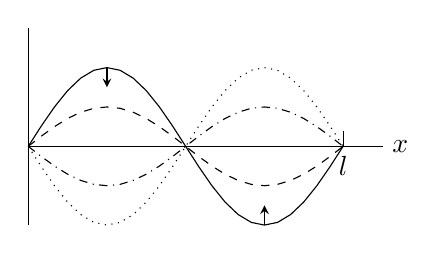
\begin{tikzpicture}
\draw(0,0)--(4.5,0)node[right]{$x$};
\draw(0,-1)--(0,1.5);
%
\draw[domain=0:360] plot ({4/360*\x},{sin(\x)});
\draw[dashed,domain=0:360] plot ({4/360*\x},{0.5*sin(\x)});
\draw[dashdotted,domain=0:360] plot ({4/360*\x},{-0.5*sin(\x)});
\draw[dotted,domain=0:360] plot ({4/360*\x},{-1*sin(\x)});
%
\draw(4,0)node[below]{$l$}--++(0,0.2);
\draw[-stealth] (1,1)--++(0,-0.25);
\draw[-stealth] (3,-1)--++(0,0.25);
\end{tikzpicture}
\caption{مختلف $t$ پر دوسرا قائمہ انداز}
\label{شکل_جزوی_مختلف_لمحات_دوسرا_قائمہ_انداز}
\end{figure}

\موٹا{تیسرا قدم۔} ظاہر ہے کہ ایک عدد حل \عددی{u_n(x,t)} عموماً ابتدائی شرائط مساوات \حوالہ{مساوات_جزوی_مساوات_موج_پ} اور مساوات \حوالہ{مساوات_جزوی_مساوات_موج_ت} کو مطمئن نہیں کر سکتا ہے۔اب چونکہ مساوات \حوالہ{مساوات_جزوی_مساوات_موج_الف} خطی اور ہم جنسی ہے لہٰذا بنیادی مسئلہ \حوالہ{مسئلہ_جزوی_بنیادی} کے تحت مساوات \حوالہ{مساوات_جزوی_مساوات_موج_الف} کی محدود تعداد کے حلوں \عددی{u_n} کا مجموعہ بھی مساوات \حوالہ{مساوات_جزوی_مساوات_موج_الف} کا حل ہو گا۔  اس طرح ایسا حل جو  ابتدائی شرائط مساوات \حوالہ{مساوات_جزوی_مساوات_موج_پ} اور مساوات \حوالہ{مساوات_جزوی_مساوات_موج_ت} کو مطمئن کرتا ہو حاصل کرنے کی خاطر ہم لامتناہی تسلسل
\begin{align}\label{مساوات_جزوی_مساوات_موج_ڈ}
u(x,t)=\sum_{n=1}^{\infty} u_n(x,t)=\sum_{n=1}^{\infty} (B_n\cos \lambda_n t+B^*_n\sin \lambda_n t)\sin \frac{n\pi}{l}x
\end{align}
پر غور کرتے ہیں۔مساوات \حوالہ{مساوات_جزوی_مساوات_موج_ڈ} اور ابتدائی شرط مساوات \حوالہ{مساوات_جزوی_مساوات_موج_پ} سے درج ذیل لکھا جا سکتا ہے۔
\begin{align}\label{مساوات_جزوی_مساوات_موج_ذ}
u(x,0)=\sum_{n=1}^{\infty} B_n\sin \frac{n\pi}{l}x=f(x)
\end{align} 
یوں اگر مساوات \حوالہ{مساوات_جزوی_مساوات_موج_ڈ} نے مساوات \حوالہ{مساوات_جزوی_مساوات_موج_پ} کو مطمئن کرنا ہو تب تب عددی سر \عددی{B_n}  اس طرح منتخب کرنے ہوں گے کہ \عددی{u(x,0)} تفاعل \عددی{f(x)} کی فوریئر سائن تسلسل ہو۔یوں  مساوات \حوالہ{مساوات_فوریئر_نصف_حلقہ_توسیع_طاق_عددی_سر} سے
\begin{align}\label{مساوات_جزوی_مساوات_موج_ر}
B_n=\frac{2}{l}\int_0^l f(x)\sin \frac{n\pi x}{l}\dif x\quad \quad \quad n=1,2,\cdots
\end{align}
حاصل ہوتا ہے۔
اسی طرح مساوات \حوالہ{مساوات_جزوی_مساوات_موج_ڈ} کا \عددی{t} کے ساتھ تفرق لے کر اور ابتدائی شرط  مساوات \حوالہ{مساوات_جزوی_مساوات_موج_ت} استعمال کرتے ہوئے درج ذیل لکھا جا سکتا ہے۔ 
\begin{align*}
\left. \frac{\partial u}{\partial t}\right|_{t=0}&=\left[\sum_{n=1}^{\infty} (-B_n\lambda_n\sin \lambda_nt+B^*_n\lambda_n\cos \lambda_nt)\sin\frac{n\pi x}{l}\right]_{t=0}\\
&=\sum_{n=1}^{\infty} B^*_n\lambda_n\sin\frac{n\pi x}{l} =g(x)
\end{align*}
یوں اگر مساوات \حوالہ{مساوات_جزوی_مساوات_موج_ڈ} نے مساوات \حوالہ{مساوات_جزوی_مساوات_موج_ت} کو مطمئن کرنا ہو تب تب عددی سر \عددی{B^*_n}  اس طرح منتخب کرنے ہوں گے کہ \عددی{t=0} پر  \عددی{\tfrac{\partial u}{\partial t}} تفاعل \عددی{g(x)} کی فوریئر سائن تسلسل ہو۔ یوں مساوات \حوالہ{مساوات_فوریئر_نصف_حلقہ_توسیع_طاق_عددی_سر} سے 
\begin{align*}
B^*_n\lambda_n=\frac{2}{l}\int_0^l g(x)\sin \frac{n\pi x}{l} \dif x
\end{align*}
اور چونکہ \عددی{\lambda_n=\tfrac{cn\pi}{l}} ہے لہٰذا
\begin{align}\label{مساوات_جزوی_مساوات_موج_ڑ}
B^*_n=\frac{2}{cn\pi}\int_0^l g(x)\sin \frac{n\pi x}{l}\dif x\quad \quad \quad n=1,2,\cdots
\end{align}
لکھا جا سکتا ہے۔

مساوات \حوالہ{مساوات_جزوی_مساوات_موج_ر} اور مساوات \حوالہ{مساوات_جزوی_مساوات_موج_ڑ} میں حاصل کیے گئے عددی سر کو مساوات \حوالہ{مساوات_جزوی_مساوات_موج_ڈ} میں پر کرنے سے حاصل تسلسل \عددی{u(x,t)}، مساوات \حوالہ{مساوات_جزوی_مساوات_موج_الف} کا ایسا حل ہو گا جو مساوات \حوالہ{مساوات_جزوی_مساوات_موج_ب}، مساوات \حوالہ{مساوات_جزوی_مساوات_موج_پ} اور مساوات \حوالہ{مساوات_جزوی_مساوات_موج_ت} کی شرائط کو مطمئن کرے گا بشرطیکہ  حاصل \عددی{u(x,t)} مرتکز ہو اور اس  کی \عددی{x} اور \عددی{t} کے ساتھ جزو در جزو  دو  درجی تفرق لینے سے حاصل تسلسل مرتکز   ہو اور ان کے مجموعے  بالترتیب \عددی{\tfrac{\partial^{\,2}u}{\partial x^2}} اور \عددی{\tfrac{\partial^{\,2}u}{\partial t^2}} کے برابر ہوں جو استمراری ہیں۔

اب تک مساوات \حوالہ{مساوات_جزوی_مساوات_موج_ڈ} محض ریاضی حل کے طور پر سامنے آیا ہے۔آئیں اس کی اصل حقیقت کو قائم کریں۔ہم اپنی آسانی کی خاطر ابتدائی رفتار \عددی{g(x)} صفر لیتے ہیں۔یوں \عددی{B^*_n=0} ہوں  گے لہٰذا مساوات \حوالہ{مساوات_جزوی_مساوات_موج_ڈ} درج ذیل صورت اختیار کرے گا۔
\begin{align}\label{مساوات_جزوی_متحرک_موج_الف}
u(x,t)=\sum_{n=1}^{\infty} B_n\cos \lambda_n t\sin\frac{n\pi x}{l},\quad \lambda_n=\frac{cn\pi}{l}
\end{align}
ہم ضمیمہ \حوالہ{ضمیمہ_مفید_معلومات} کا کلیہ \حوالہ{مساوات_ضمیمہ_مفید_گیارہ} استعمال کرتے ہوئے
\begin{align*}
\cos \frac{cn\pi}{l}t\,\sin\frac{n\pi}{l}x=\frac{1}{2}\big[\sin\big\{\frac{n\pi}{l}(x-ct)\big\}+\sin\big\{\frac{n\pi}{l}(x+ct)\big\}\big]
\end{align*}
لکھ سکتے ہیں جس کو  مساوات \حوالہ{مساوات_جزوی_متحرک_موج_الف}  میں پر کرتے ہوئے درج ذیل ملتا ہے۔
\begin{align*}
u(x,t)=\frac{1}{2}\sum_{n=1}^{\infty}B_n \sin\big\{\frac{n\pi}{l}(x-ct)\big\}+\frac{1}{2}\sum_{n=1}^{\infty}B_n \sin\big\{\frac{n\pi}{l}(x+ct)\big\}
\end{align*}
آپ دیکھ سکتے ہیں کہ مساوات \حوالہ{مساوات_جزوی_مساوات_موج_ذ} میں \عددی{x} کی جگہ \عددی{x-ct} اور \عددی{x+ct} پر کرنے سے یہی دو تسلسل حاصل ہوتے ہیں لہٰذا ہم درج ذیل لکھ سکتے ہیں
\begin{align}\label{مساوات_جزوی_متحرک_موج_ب}
u(x,t)=\frac{1}{2}[f^*(x-ct)+f^*(x+ct)]
\end{align}
جہاں \عددی{f} کی طاق دوری توسیع جس کا دوری عرصہ \عددی{2l} ہو تفاعل \عددی{f^*} ہے (شکل \حوالہ{شکل_جزوی_طاق_توسیع})۔چونکہ وقفہ \عددی{0\le x\le l} پر ابتدائی انحراف \عددی{f(x)} استمراری ہے جبکہ  \عددی{x=0} اور \عددی{x=l} پر انحراف صفر ہے لہٰذا مساوات \حوالہ{مساوات_جزوی_متحرک_موج_ب} سے ظاہر ہے کہ \عددی{u(x,t)} دونوں متغیرات \عددی{x} اور \عددی{t} کی تمام قیمتوں پر استمراری ہو گا۔مساوات \حوالہ{مساوات_جزوی_متحرک_موج_ب} کا تفرق لیتے ہوئے ہم دیکھتے ہیں کہ یہ مساوات \حوالہ{مساوات_جزوی_مساوات_موج_الف} کا حل ہے بشرطیکہ  وقفہ \عددی{0<x<l} پر \عددی{f(x)} دو مرتبہ قابل تفرق ہو اور \عددی{x=0} اور \عددی{x=l} پر اس کے یک طرفہ دو درجی تفرق پائے جاتے ہوں جن کی قیمت صفر کے برابر ہو۔اس طرح یہ حقیقت قائم ہوتی ہے کہ ان شرائط پر پورا اترتا ہوا تسلسل \عددی{u(x,t)} مساوات \حوالہ{مساوات_جزوی_مساوات_موج_الف} کا ایسا حل ہو گا جو  مساوات \حوالہ{مساوات_جزوی_مساوات_موج_ب}، مساوات \حوالہ{مساوات_جزوی_مساوات_موج_پ} اور مساوات \حوالہ{مساوات_جزوی_مساوات_موج_ت} کی شرائط کو مطمئن کرتا ہے ۔
\begin{figure}
\centering
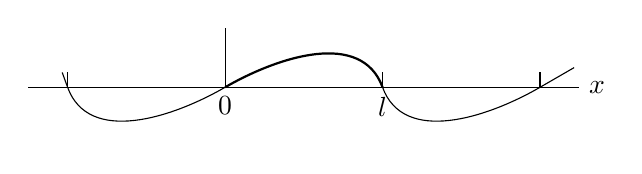
\begin{tikzpicture}
\draw(-2.5,0)--(4.5,0)node[right]{$x$};
\draw(0,0)node[below]{$0$}--(0,0.75);
\draw[thick](0,0) to [out=30,in=110] ++(2,0)node[below]{$l$};
\draw(2,0) to [out=-70,in=-150]++(2,0) --++(30:0.5);
\draw(0,0) to [out=-150,in=-70]++(-2,0)--++(110:0.2);
\draw(-2,0)--++(0,0.2);
\draw(2,0)--++(0,0.2);
\draw(4,0)--++(0,0.2);
\end{tikzpicture}
\caption{$f(x)$ کی طاق توسیع}
\label{شکل_جزوی_طاق_توسیع}
\end{figure}

اگر \عددی{f'(x)} اور \عددی{f''(x)} محض ٹکڑوں میں استمراری (حصہ \حوالہ{حصہ_لاپلاس_بدل_الٹ_بدل_خطیت}) ہوں، یا اگر وقفہ کے سروں پر یک طرفہ تفرقات غیر صفر ہوں تب ہر ایک \عددی{t} کے لئے محدود تعداد کی \عددی{x} قیمتوں پر مساوات \حوالہ{مساوات_جزوی_مساوات_موج_الف} کے \عددی{u} کی دو درجی تفرقات غیر معین ہوں گے۔ان نقطوں کے علاوہ باقی تمام نقطوں پر \عددی{u} مساوات موج کو مطمئن کرے گی لہٰذا ہم \عددی{u(x,t)} کو وسیع معنوں میں مسئلے کا حل تصور کر سکتے ہیں۔مثال کے طور پر تکونی ابتدائی انحراف کی صورت میں حاصل حل اس نوعیت کا ہو گا۔
\begin{figure}
\centering
\begin{tikzpicture}
\draw(-2,0)--(7,0)node[right]{$x$};
\draw(0,-1.7)--(0,1);
%
\draw(-2,-1) to [out=-20,in=-135]++(2,1)node[ocirc]{} to [out=45,in=180]++(1,1)node[above]{$f^*(x)$} to [out=0,in=180]++(1,-0.7) to [out=0,in=180]++(0.5,0.2) to [out=0,in=90]++(0.5,-0.5);
\draw[dashed](1.5,-1) to [out=-20,in=-135]++(2,1)to [out=45,in=180]++(1,1)node[above,solid]{$f^*(x-ct)$} to [out=0,in=180]++(1,-0.7) to [out=0,in=180]++(0.5,0.2) to [out=0,in=90]++(0.5,-0.5);
\draw(3.5,0)--++(0,-1.7);
\draw[stealth-stealth] (0,-1.7)--++(3.5,0)node[pos=0.5,fill=white]{$ct$};
\end{tikzpicture}
\caption{مساوات \حوالہ{مساوات_جزوی_متحرک_موج_ب} کی معنی}
\label{شکل_جزوی_موج_حرکت}
\end{figure}

آئیں   مساوات \حوالہ{مساوات_جزوی_متحرک_موج_ب} کی طبعی معنی سمجھتے ہیں۔جیسا شکل \حوالہ{شکل_جزوی_موج_حرکت} میں دکھایا گیا ہے، \عددی{f^*(x)} کی ترسیم کو \عددی{ct} اکائیاں دائیں منتقل کرنے سے \عددی{f^*(x-ct)} کی ترسیم حاصل ہوتی ہے۔ اس کا مطلب ہے کہ \عددی{f^*(x-ct),\,\, (c>0)} ایسی موج کو ظاہر کرتا ہے جو بڑھتے \عددی{t} کے ساتھ دائیں جانب کو حرکت کرتی ہے۔اسی طرح \عددی{f^*(x+ct),\,\, (c>0)} ایسی موج کو ظاہر کرتا ہے جو بڑھتے \عددی{t} کے ساتھ بائیں جانب کو حرکت کرتی ہے اور \عددی{u(x,t)} ان دونوں کا مجموعہ ہے۔

%======================

\begin{figure}
\centering
\begin{tikzpicture}
\pgfmathsetmacro{\kks}{-1.5}
\pgfmathsetmacro{\khs}{-5}
%
\pgfmathsetmacro{\ang}{30}
\pgfmathsetmacro{\l}{1}
\pgfmathsetmacro{\h}{\l*tan(\ang)}
%
\pgfmathsetmacro{\a}{1*\l}
\pgfmathsetmacro{\b}{2*\l-\a}
\pgfmathsetmacro{\aa}{\a/cos(\ang)}
\pgfmathsetmacro{\bb}{\b/cos(\ang)}
%
\draw(0,0)node[below]{$0$}--(2,0)node[below]{$l$};
\draw(0,0)--++(0,0.2);
\draw(2,0)--++(0,0.2);
%
\draw[thick](\a,\h)--++(-180+\ang:\aa);
\draw[thick](\a,\h)--++(-\ang:\bb)node[pos=0.5,above right]{$\tfrac{1}{2}f^*(x)$};
%=================
\begin{scope}[shift={(\khs,0)}]
\pgfmathsetmacro{\hh}{2*\h-2*(\l-\a)*tan(\ang)}
%
\draw(0,0)node[below]{$0$}--(2,0)node[below]{$l$};
\draw(0,0)--++(0,0.2);
\draw(2,0)--++(0,0.2);
%
\draw[thick] (0,0)--(\a,\hh)--(2*\l-\a,\hh)--(2*\l,0);
\draw(\a,\hh)node[left]{$u(x,0)$};
\draw(0,\hh/2)node[left]{$t=0$};
\end{scope}
%=========================
%==========================
\begin{scope}[shift={(0,1*\kks)}]
\pgfmathsetmacro{\a}{2/3*\l}
\pgfmathsetmacro{\b}{2*\l-\a}
\pgfmathsetmacro{\aa}{\a/cos(\ang)}
\pgfmathsetmacro{\bb}{\b/cos(\ang)}
%
\draw(0,0)--(2,0);
\draw(0,0)--++(0,0.2);
\draw(2,0)--++(0,0.2);
%
\draw[thick](\a,\h)--++(-180+\ang:\aa);
\draw[thick](\a,\h)--++(-\ang:\bb);
%
\draw[thick,dashed] (\b,\h)--++(-\ang:\aa);
\draw[thick,dashed](\b,\h)--++(-180+\ang:\bb);
%
\draw[-stealth] (\a,1.2*\h)--++(-0.5,0)node[left]{$\tfrac{1}{2}f^*(x+\tfrac{l}{5})$};
\draw[-stealth,dashed] (2*\l-\a,1.2*\h)--++(0.5,0)node[right]{$\tfrac{1}{2}f^*(x-\tfrac{l}{5})$};
%=================
\begin{scope}[shift={(\khs,0)}]
\pgfmathsetmacro{\hh}{2*\h-2*(\l-\a)*tan(\ang)}
%
\draw(0,0)--(2,0);
\draw(0,0)--++(0,0.2);
\draw(2,0)--++(0,0.2);
%
\draw[thick] (0,0)--(\a,\hh)--(2*\l-\a,\hh)--(2*\l,0);
\draw(0,\hh/2)node[left]{$t=\tfrac{l}{5c}$};
\end{scope}
\end{scope}
%============================
%==================================
\begin{scope}[shift={(0,2*\kks)}]
\pgfmathsetmacro{\a}{1/3*\l}
\pgfmathsetmacro{\b}{2*\l-\a}
\pgfmathsetmacro{\aa}{\a/cos(\ang)}
\pgfmathsetmacro{\bb}{\b/cos(\ang)}
%
\draw(0,0)--(2,0);
\draw(0,0)--++(0,0.2);
\draw(2,0)--++(0,0.2);
%
\draw[thick](\a,\h)--++(-180+\ang:\aa);
\draw[thick](\a,\h)--++(-\ang:\bb);
%
\draw[thick,dashed] (\b,\h)--++(-\ang:\aa);
\draw[thick,dashed](\b,\h)--++(-180+\ang:\bb);
\draw[] (0,\h/2)node[left]{$\tfrac{1}{2}f^*(x+\tfrac{2l}{5})$};
\draw[] (2*\l,\h/2)node[right]{$\tfrac{1}{2}f^*(x-\tfrac{2l}{5})$};
%=================
\begin{scope}[shift={(\khs,0)}]
\pgfmathsetmacro{\hh}{2*\h-2*(\l-\a)*tan(\ang)}
%
\draw(0,0)--(2,0);
\draw(0,0)--++(0,0.2);
\draw(2,0)--++(0,0.2);
%
\draw[thick] (0,0)--(\a,\hh)--(2*\l-\a,\hh)--(2*\l,0);
\draw(0,\hh/2)node[left]{$t=\tfrac{2l}{5c}$};
\end{scope}
\end{scope}
%======================
%=============================
\begin{scope}[shift={(0,3*\kks)}]
\pgfmathsetmacro{\a}{0*\l}
\pgfmathsetmacro{\b}{2*\l-\a}
\pgfmathsetmacro{\aa}{\a/cos(\ang)}
\pgfmathsetmacro{\bb}{\b/cos(\ang)}
%
\draw(0,0)--(2,0);
\draw(0,0)--++(0,0.2);
\draw(2,0)--++(0,0.2);
%
\draw[thick](\a,\h)--++(-180+\ang:\aa);
\draw[thick](\a,\h)--++(-\ang:\bb);
%
\draw[thick,dashed] (\b,\h)--++(-\ang:\aa);
\draw[thick,dashed](\b,\h)--++(-180+\ang:\bb);
\draw[] (0,\h/2)node[left]{$\tfrac{1}{2}f^*(x+\tfrac{l}{2})$};
\draw[] (2*\l,\h/2)node[right]{$\tfrac{1}{2}f^*(x-\tfrac{l}{2})$};
\begin{scope}[shift={(\khs,0)}]
\pgfmathsetmacro{\hh}{2*\h-2*(\l-\a)*tan(\ang)}
%
\draw(0,0)--(2,0);
\draw(0,0)--++(0,0.2);
\draw(2,0)--++(0,0.2);
%
\draw[thick] (0,0)--(\a,\hh)--(2*\l-\a,\hh)--(2*\l,0);
\draw(0,\hh/2)node[left]{$t=\tfrac{l}{2c}$};
\end{scope}
\end{scope}
%======================================
%======================================
%===================================
\begin{scope}[shift={(0,4*\kks)}]
\pgfmathsetmacro{\a}{1/3*\l}
\pgfmathsetmacro{\b}{2*\l-\a}
\pgfmathsetmacro{\aa}{\a/cos(\ang)}
\pgfmathsetmacro{\bb}{\b/cos(\ang)}
%
\draw(0,0)--(2,0);
\draw(0,0)--++(0,0.2);
\draw(2,0)--++(0,0.2);
%
\draw[thick,dashed](\a,-\h)--++(180-\ang:\aa);
\draw[thick,dashed](\a,-\h)--++(\ang:\bb);
%
\draw[thick] (\b,-\h)--++(\ang:\aa);
\draw[thick](\b,-\h)--++(180-\ang:\bb);
\draw[] (0,\h/2)node[left]{$\tfrac{1}{2}f^*(x+\tfrac{3l}{5})$};
\draw[] (2*\l,\h/2)node[right]{$\tfrac{1}{2}f^*(x-\tfrac{3l}{5})$};
\begin{scope}[shift={(\khs,0)}]
\pgfmathsetmacro{\hh}{2*\h-2*(\l-\a)*tan(\ang)}
%
\draw(0,0)--(2,0);
\draw(0,0)--++(0,0.2);
\draw(2,0)--++(0,0.2);
%
\draw[thick] (0,0)--(\a,-\hh)--(2*\l-\a,-\hh)--(2*\l,0);
\draw(0,0)node[left]{$t=\tfrac{3l}{5c}$};
\end{scope}
\end{scope}
%==================================
%====================================
\begin{scope}[shift={(0,5*\kks)}]
\pgfmathsetmacro{\a}{2/3*\l}
\pgfmathsetmacro{\b}{2*\l-\a}
\pgfmathsetmacro{\aa}{\a/cos(\ang)}
\pgfmathsetmacro{\bb}{\b/cos(\ang)}
%
\draw(0,0)--(2,0);
\draw(0,0)--++(0,0.2);
\draw(2,0)--++(0,0.2);
%
\draw[thick,dashed](\a,-\h)--++(180-\ang:\aa);
\draw[thick,dashed](\a,-\h)--++(\ang:\bb);
%
\draw[thick] (\b,-\h)--++(\ang:\aa);
\draw[thick](\b,-\h)--++(180-\ang:\bb);
\draw[] (0,\h/2)node[left]{$\tfrac{1}{2}f^*(x+\tfrac{4l}{5})$};
\draw[] (2*\l,\h/2)node[right]{$\tfrac{1}{2}f^*(x-\tfrac{4l}{5})$};
\begin{scope}[shift={(\khs,0)}]
\pgfmathsetmacro{\hh}{2*\h-2*(\l-\a)*tan(\ang)}
%
\draw(0,0)--(2,0);
\draw(0,0)--++(0,0.2);
\draw(2,0)--++(0,0.2);
%
\draw[thick] (0,0)--(\a,-\hh)--(2*\l-\a,-\hh)--(2*\l,0);
\draw(0,0)node[left]{$t=\tfrac{4l}{5c}$};
\end{scope}
\end{scope}
%==========================
%============================
\begin{scope}[shift={(0,6*\kks)}]
\pgfmathsetmacro{\a}{1*\l}
\pgfmathsetmacro{\b}{2*\l-\a}
\pgfmathsetmacro{\aa}{\a/cos(\ang)}
\pgfmathsetmacro{\bb}{\b/cos(\ang)}
%
\draw(0,0)--(2,0);
\draw(0,0)--++(0,0.2);
\draw(2,0)--++(0,0.2);
%
\draw[thick] (\b,-\h)--++(\ang:\aa);
\draw[thick](\b,-\h)--++(180-\ang:\bb);
\draw[] (\a,-\h/2)++(-1,0)node[left]{$\substack{\tfrac{1}{2}f^*(x+l)\\=\tfrac{1}{2}f^*(x-l)}$};
\begin{scope}[shift={(\khs,0)}]
\pgfmathsetmacro{\hh}{2*\h-2*(\l-\a)*tan(\ang)}
%
\draw(0,0)--(2,0);
\draw(0,0)--++(0,0.2);
\draw(2,0)--++(0,0.2);
%
\draw[thick] (0,0)--(\a,-\hh)--(2*\l-\a,-\hh)--(2*\l,0);
\draw(0,0)node[left]{$t=\tfrac{l}{c}$};
\end{scope}
\end{scope}
\end{tikzpicture}
\caption{مثال \حوالہ{مثال_جزوی_تکونی_انحراف} کا مختلف لمحات پر دائیں کو اور بائیں کو حرکت کرتے اجزاء اور ان کا مجموعہ حل $u(x,t)$}
\label{شکل_مثال_جزوی_تکونی_انحراف}
\end{figure}
%================
\ابتدا{مثال}\شناخت{مثال_جزوی_تکونی_انحراف}\quad تکونی ابتدائی انحراف کی صورت میں تار کی ارتعاش\\
مساوات موج \حوالہ{مساوات_جزوی_مساوات_موج_الف} کا حل تکونی ابتدائی انحراف
\begin{align*}
f(x)=
\begin{cases}
\frac{2k}{l}x&0<x<\frac{l}{2}\\
\frac{2k}{l}(l-x)&\frac{l}{2}<x<l
\end{cases}
\end{align*}
اور ابتدائی رفتار صفر \عددی{g(x)=0} کی صورت میں حاصل کریں۔\\
حل: چونکہ \عددی{g(x)\equiv 0} ہے لہٰذا مساوات \حوالہ{مساوات_جزوی_متحرک_موج_الف} میں \عددی{B^*_n=0} ہو گا جبکہ \عددی{B_n} کو صفحہ \حوالہصفحہ{مساوات_فوریئر_تکونی_دھڑکن_عددی_سر_ب} پر مساوات \حوالہ{مساوات_فوریئر_تکونی_دھڑکن_عددی_سر_ب} دے گی۔یوں  مساوات \حوالہ{مساوات_جزوی_متحرک_موج_الف} درج ذیل صورت اختیار کرے گی۔
\begin{align*}
u(x,t)=\frac{8k}{\pi^2}\big[\frac{1}{1^2}\sin \frac{\pi}{l}x\cos\frac{\pi c}{l}t-\frac{1}{3^2}\sin \frac{3\pi}{l}x\cos\frac{3\pi c}{l}t+-\cdots\big]
\end{align*}
اس حل کی ترسیم کھینچنے کی خاطر ہم \عددی{u(x,0)=f(x)} سے شروع کرتے ہوئے مساوات \حوالہ{مساوات_جزوی_متحرک_موج_ب} کی مدد لیتے ہیں۔یوں شکل \حوالہ{شکل_مثال_جزوی_تکونی_انحراف} حاصل ہوتی ہے۔
\انتہا{مثال}
%======================

\حصہء{سوالات}
سوال \حوالہ{سوال_جزوی_انحراف_تار_الف} تا سوال \حوالہ{سوال_جزوی_انحراف_تار_ب} میں تار کی لمبائی \عددی{l=\pi} اور \عددی{c^2=\tfrac{T}{\rho}=1} ہے۔تار کے سرے ٹھوس نقطوں کے ساتھ باندھے گئے ہیں۔ابتدائی رفتار صفر جبکہ ابتدائی انحراف \عددی{f(x)} سوال میں دی گئی ہے۔ارتعاش پذیر تار کا انحراف \عددی{u(x,t)} دریافت کریں۔

%==================
\ابتدا{سوال}\شناخت{سوال_جزوی_انحراف_تار_الف}\quad
$0.02\sin x$\\
جواب:\quad 
$u=0.02\cos t\sin x$
\انتہا{سوال}
%====================
\ابتدا{سوال}\quad
$k\sin 2x$\\
جواب:\quad
$u=k\cos 2t\sin 2x$
\انتہا{سوال}
%====================
\ابتدا{سوال}\quad
$k(\sin x-\sin 2x)$\\
جواب:\quad
$u=k(\cos t\sin x-\cos 2t\sin 2x)$
\انتہا{سوال}
%====================
\ابتدا{سوال}\شناخت{سوال_جزوی_شکل_انحراف_الف}\quad شکل \حوالہ{شکل_سوال_جزوی_شکل_انحراف_الف}-الف \\
جواب:\quad
$\tfrac{9\sqrt{3}k}{2\pi^2}(\tfrac{1}{1^2}\cos t\sin x+\tfrac{1}{2^2}\cos2t\sin 2x-\tfrac{1}{4^2}\cos 4t\sin 4x\cdots)$
%
\begin{figure}
\centering
\begin{subfigure}{0.3\textwidth}
\centering
\begin{tikzpicture}
\draw(0,0)--(2.5,0)node[right]{$x$};
\draw(0,0)--(0,1);
\draw[thick](0,0)--(2/3,0.5)--(2,0);
\draw(2/3,0)node[below]{$\tfrac{\pi}{3}$}--++(0,0.2);
\draw(2,0)node[below]{$\pi$}--++(0,0.2);
\draw[dashed](0,0.5)node[left,solid]{$0.05$}--++(2/3,0);
\end{tikzpicture}
\caption*{(الف)}
\end{subfigure}%
\begin{subfigure}{0.3\textwidth}
\centering
\begin{tikzpicture}
\draw(0,0)--(2.5,0)node[right]{$x$};
\draw(0,-1)--(0,1);
\draw[thick](0,0)--(0.5,0.5)--(1.5,-0.5)--(2,0);
\draw(0.5,0)node[below]{$\tfrac{\pi}{4}$}--++(0,0.2);
\draw(1,0)node[below]{$\tfrac{\pi}{2}$}--++(0,0.2);
\draw(1.5,0)--++(0,0.2)node[above]{$\tfrac{3\pi}{2}$};
\draw(2,0)node[below]{$\pi$}--++(0,0.2);
\draw[](0,0.5)node[left]{$\tfrac{\pi}{40}$}--++(0.2,0);
\draw[](0,-0.5)node[left]{$-\tfrac{\pi}{40}$}--++(0.2,0);
\end{tikzpicture}
\caption*{(ب)}
\end{subfigure}%
\begin{subfigure}{0.3\textwidth}
\centering
\begin{tikzpicture}
\draw(0,0)--(2.5,0)node[right]{$x$};
\draw(0,0)--(0,1);
\draw[thick](0,0)--(0.5,0.5)--(1,0)--(2,0);
\draw(0.5,0)node[below]{$\tfrac{\pi}{4}$}--++(0,0.2);
\draw(1,0)node[below]{$\tfrac{\pi}{2}$}--++(0,0.2);
\draw(2,0)node[below]{$\pi$}--++(0,0.2);
\draw[dashed](0,0.5)node[left,solid]{$k$}--(0.5,0.5);
\end{tikzpicture}
\caption*{(پ)}
\end{subfigure}%
\caption{اشکال برائے سوالات \حوالہ{سوال_جزوی_شکل_انحراف_الف}، \حوالہ{سوال_جزوی_شکل_انحراف_ب} اور \حوالہ{سوال_جزوی_شکل_انحراف_پ}}
\label{شکل_سوال_جزوی_شکل_انحراف_الف}
\end{figure}
\انتہا{سوال}
%===============
\ابتدا{سوال}\شناخت{سوال_جزوی_شکل_انحراف_ب}\quad شکل \حوالہ{شکل_سوال_جزوی_شکل_انحراف_الف}-ب \\
جواب:\quad
$\tfrac{4}{5\pi}(\tfrac{1}{2^2}\cos 2t\sin 2x-\tfrac{1}{6^2}\cos 6t\sin 6x+\tfrac{1}{10^2}\cos 10t\sin 10x\cdots)$
\انتہا{سوال}
%========================
\ابتدا{سوال}\شناخت{سوال_جزوی_شکل_انحراف_پ}\quad شکل \حوالہ{شکل_سوال_جزوی_شکل_انحراف_الف}-پ\\
جواب:\quad
$\tfrac{4k}{\pi^2}[2(\sqrt{2}-1)\cos t\sin x +\cos 2t\sin 2x-2(\sqrt{2}-\tfrac{1}{9})\cos 3t\sin 3x\cdots]$
\انتہا{سوال}
%========================
\ابتدا{سوال}\quad
$kx(x-\pi)$\\
جواب:\quad
$\tfrac{8k}{\pi}(\tfrac{1}{1^2}\cos t\sin x-\tfrac{1}{3^2}\cos 3t\sin 3x-\tfrac{1}{5^2}\cos 5t\sin 5x\cdots)$
\انتہا{سوال}
%======================
\ابتدا{سوال}\quad 
\begin{align*}
f(x)=
\begin{cases}
kx^2&0<x<\frac{\pi}{2}\\
k(x-\pi)^2&\frac{\pi}{2}<x<\pi
\end{cases}
\end{align*}
جواب:\quad
$4k[(1-\tfrac{2}{\pi})\cos t\sin x-\tfrac{1}{9}(1+\tfrac{2}{3\pi})\cos 3t\sin 3x\cdots]$
\انتہا{سوال}
%===========================
\ابتدا{سوال}\شناخت{سوال_جزوی_انحراف_تار_ب}\quad 
\begin{align*}
f(x)=
\begin{cases}
kx^2&0<x<\frac{\pi}{2}\\
-k(x-\pi)^2&\frac{\pi}{2}<x<\pi
\end{cases}
\end{align*}
جواب:\quad
$k(\tfrac{\pi}{2}-\tfrac{2}{\pi})\cos 2t\sin 2x+\tfrac{k\pi}{4}\cos 4t\sin 4x+k(\tfrac{\pi}{6}-\tfrac{2}{27\pi})\cos 6t\sin 6x\cdots$
\انتہا{سوال}
%===========================
سوال \حوالہ{سوال_جزوی_ابتدائی_رفتار_اور_انحراف_الف} تا سوال \حوالہ{سوال_جزوی_ابتدائی_رفتار_اور_انحراف_ب} میں \عددی{c^2=1} ہے، تار کی لمبائی \عددی{l=\pi} ہے اور تار کے سرے ٹھوس نقطوں سے بندھے ہیں۔ابتدائی رفتار \عددی{g(x)} اور ابتدائی انحراف \عددی{f(x)} ہیں۔ارتعاش پذیر تار کی انحراف \عددی{u(x,t)} دریافت کریں۔

%============
\ابتدا{سوال}\شناخت{سوال_جزوی_ابتدائی_رفتار_اور_انحراف_الف}\quad
$f=0,\quad g=kx \quad (0\le x\le \tfrac{\pi}{2});\quad g(x)=k(\pi-x)\quad (\tfrac{\pi}{2}\le x\le \pi)$\\
جواب:\quad
$\tfrac{4k}{\pi}(\tfrac{1}{1^3}\sin t\sin x-\tfrac{1}{3^3}\sin 3t\sin 3x+\tfrac{1}{5^3}\sin 5t\sin 5x\cdots)$
\انتہا{سوال}
%==================
\ابتدا{سوال}\quad
$f=0,\quad g=k\sin 3x$\\
جواب:\quad
$\tfrac{k}{3}\sin 3t\sin 3x$
\انتہا{سوال}
%==================
\ابتدا{سوال}\شناخت{سوال_جزوی_ابتدائی_رفتار_اور_انحراف_ب}\quad
$f=k\sin 2x,\quad g=-k\sin 2x$\\
جواب:\quad
$-\tfrac{k}{2}\sin 2t\sin 2x$
\انتہا{سوال}
%==================
\ابتدا{سوال}\quad
تناو \عددی{T} چار گنا کرنے سے بنیادی انداز کی تعدد پر کیا اثر ہو گا؟\\
جواب:\quad چونکہ \عددی{c^2=\tfrac{T}{\rho}} ہے لہٰذا \عددی{T} چار گنا کرنے سے \عددی{c} دگنا ہو گا جس سے بنیادی انداز کی تعدد دگنی ہو گی۔
\انتہا{سوال}
%=====================
\ابتدا{سوال}\quad
تار کی لمبائی  چار گنا کرنے سے بنیادی انداز کی تعدد پر کیا اثر ہو گا؟\\
جواب:\quad بنیادی انداز کی تعدد چار گنا کم ہو گی۔
\انتہا{سوال}
%=====================
سوال \حوالہ{سوال_جزوی_علیحدگی_متغیرات_الف} تا سوال \حوالہ{سوال_جزوی_علیحدگی_متغیرات_ب} میں دیے گئے جزوی تفرقی مساوات کو علیحدگی متغیرات کے طریقہ سے حل کریں۔

%=================
\ابتدا{سوال}\شناخت{سوال_جزوی_علیحدگی_متغیرات_الف}\quad
$u_x+u_y=0$\\
جواب:\quad
$u=ce^{k(x+y)}$
\انتہا{سوال}
%========================
\ابتدا{سوال}\quad
$u_x-u_y=0$\\
جواب:\quad
$u=ce^{k(x-y)}$
\انتہا{سوال}
%========================
\ابتدا{سوال}\quad
$xu_x-yu_y=0$\\
جواب:\quad
$u=kxy$
\انتہا{سوال}
%========================
\ابتدا{سوال}\quad
$u_x-yu_y=0$\\
جواب:\quad
$u=cy^ke^{kx}$
\انتہا{سوال}
%========================
\ابتدا{سوال}\quad
$yu_x-xu_y=0$\\
جواب:\quad
$u=ce^{k(x^2+y^2)}$
\انتہا{سوال}
%========================
\ابتدا{سوال}\quad
$u_x+u_y=2(x+y)u$\\
جواب:\quad
$u=ce^{x^2+y^2+k(x-y)}$
\انتہا{سوال}
%========================
\ابتدا{سوال}\quad
$u_{xx}+u_{yy}=0$\\
جواب:\quad
$u=(A\cos kx+B\sin kx)(Ce^{ky}+De^{-ky})$
\انتہا{سوال}
%========================
\ابتدا{سوال}\شناخت{سوال_جزوی_علیحدگی_متغیرات_ب}\quad
$u_{xy}-u=0$\\
جواب:\quad
$u=ce^{x+y}$
\انتہا{سوال}
%========================
سوال \حوالہ{سوال_جزوی_تار_جبری_الف} تا سوال \حوالہ{سوال_جزوی_تار_جبری_ٹ} \موٹا{لچکدار تار کی جبری ارتعاش} پر مبنی ہیں۔

%====================
\ابتدا{سوال}\شناخت{سوال_جزوی_تار_جبری_الف}\quad لچک دار تار کی جبری ارتعاش کا الجبرائی نمونہ درج ذیل جزوی تفرقی مساوات  ہے جہاں اکائی لمبائی پر  بیرونی قوت \عددی{P(x,t)}  تار کے عمودی عمل کرتا ہے۔
\begin{align}\label{مساوات_جزوی_تار_جبری_الف}
u_{tt}=c^2u_{xx}+\frac{P}{\rho}
\end{align} 
دیے گئے مسئلے سے اس جزوی تفرقی مساوات کو حاصل کریں۔
\انتہا{سوال}
%====================
\ابتدا{سوال}\شناخت{سوال_جزوی_تار_جبری_ب}\quad
سائن نما بیرونی قوت \عددی{P=A\rho \sin \omega t} کی صورت میں درج ذیل ثابت کریں
\begin{align*}
\frac{P}{\rho}=A\sin \omega t=\sum_{n=1}^{\infty} k_n(t)\sin \frac{n\pi x}{l}
\end{align*}
جہاں 
$k_n(t)=\tfrac{2A}{n\pi}(1-\cos n\pi)\sin \omega t$
 ہے۔یوں جفت \عددی{n} کی صورت میں \عددی{k_n=0} اور طاق \عددی{n} کی صورت میں 
$k_n=\tfrac{4A}{n\pi}\sin \omega t$
ہو گا۔مزید ثابت کریں کہ مساوات \حوالہ{مساوات_جزوی_مساوات_موج_الف} میں
\begin{align*}
u(x,t)=\sum_{n=1}^{\infty} G(t)\sin \frac{n\pi x}{l}
\end{align*}
پر کرنے سے درج ذیل ملتا ہے۔
\begin{align*}
\ddot{G}_n+\lambda^2_n G_n=0,\quad \lambda_n=\frac{cn\pi}{l}
\end{align*}
\انتہا{سوال}
%===================
\ابتدا{سوال}\شناخت{سوال_جزوی_تار_جبری_پ}\quad
ثابت کریں کہ  سوال \حوالہ{سوال_جزوی_تار_جبری_ب} کے \عددی{\tfrac{P}{\rho}} اور \عددی{u} کو مساوات \حوالہ{مساوات_جزوی_تار_جبری_الف} میں پر کرنے سے درج ذیل حاصل ہوتا ہے۔
\begin{align*}
\ddot{G}_n+\lambda^2_nG_n=\frac{2A}{n\pi}(1-\cos n\pi)\sin\omega t,\quad \quad \lambda_n=\frac{cn\pi}{l}
\end{align*}  
ثابت کریں کہ \عددی{\lambda^2_n\ne \omega^2} کی صورت میں اس کا حل درج ذیل ہو گا۔
\begin{align*}
G_n(t)=B_n\cos\lambda_nt+B^*_n\sin\lambda_nt+\frac{2A(1-\cos n\pi)}{n\pi(\lambda^2_n-\omega^2)}\sin \omega t
\end{align*}
\انتہا{سوال}
%========================
\ابتدا{سوال}\شناخت{سوال_جزوی_تار_جبری_ت}\quad
ایسے \عددی{B_n} اور \عددی{B^*_n} دریافت کریں کہ \عددی{u} ابتدائی شرائط \عددی{u(x,0)=f(x)} اور \عددی{u_t(x,0)=0} کو مطمئن کرے (سوال \حوالہ{سوال_جزوی_تار_جبری_پ})۔
\انتہا{سوال}
%=====================
\ابتدا{سوال}\شناخت{سوال_جزوی_تار_جبری_ٹ}\quad
ثابت کریں کہ گمک \عددی{\lambda_n=\omega} کی صورت میں درج ذیل ہو گا۔
\begin{align*}
G_n(t)=B_n\cos \omega t+B^*_n\sin\omega t-\frac{A}{n\pi \omega}(1-\cos n\pi)t\cos \omega t
\end{align*}
\انتہا{سوال}
%=========================

\حصہ{مساوات موج کا دا لومبیغ حل}
گزشتہ حصہ میں مساوات موج
\begin{align}\label{مساوات_جزوی_موج_مساوات_الف}
\frac{\partial^{\,2}u}{\partial t^2}=c^2\frac{\partial^{\,2}u}{\partial x^2}
\end{align}
کا حل مساوات \حوالہ{مساوات_جزوی_متحرک_موج_ب} حاصل کیا گیا۔یہی حل نہایت آسانی سے مساوات \حوالہ{مساوات_جزوی_موج_مساوات_الف} کا موزوں بدل لیتے ہوئے حاصل کیا جا سکتا ہے۔یوں نئے غیر تابع متغیرات\حاشیہد{یہاں بتلاتا چلوں کہ جزوی تفرقی مساوات کا عمومی نظریہ اس طرح کے تبادل حاصل کرنے کی قدم با قدم ترکیب پیش کرتی ہے۔}
\begin{align}\label{مساوات_جزوی_موج_مساوات_ب}
v=x+ct,\quad z=x-ct
\end{align}
متعارف کرتے ہوئے \عددی{u} کو متغیرات \عددی{v} اور \عددی{z} کا تفاعل لکھتے ہیں۔اس طرح مساوات \حوالہ{مساوات_جزوی_موج_مساوات_الف} میں تفرقات اب \عددی{v} اور \عددی{z} کے لحاظ سے زنجیری ترکیب (حصہ \حوالہ{حصہ_الاحصاء_زنجیری_ترکیب})  کی مدد سے لکھے جائیں گے۔جزوی تفرق کو زیر نوشت سے ظاہر کرتے ہوئے  مساوات \حوالہ{مساوات_جزوی_موج_مساوات_ب} سے \عددی{v_x=1} اور \عددی{z_x=1} لکھے جائیں گے۔ہم اپنی آسانی کے لئے ہم \عددی{v} اور \عددی{z} متغیرات کے تفاعل کو بھی \عددی{u} سے ظاہر کرتے ہیں۔اس طرح درج ذیل لکھا جا سکتا ہے۔
\begin{align*}
u_x=u_vv_x+u_zz_x=u_v+u_z
\end{align*}
دائیں ہاتھ پر زنجیری ترکیب لاگو کرتے ہوئے اور \عددی{v_x=1} اور \عددی{z_x=1} پر کرتے ہوئے
\begin{align*}
u_{xx}=(u_v+u_z)_x=(u_v+u_z)_vv_x+(u_v+u_z)_zz_x=u_{vv}+2u_{vz}+u_{zz}
\end{align*}
ملتا ہے۔مساوات \حوالہ{مساوات_جزوی_موج_مساوات_الف} کی دوسری تفرق کو بھی اسی طرح لکھتے ہیں۔
\begin{align*}
u_{tt}=c^2(u_{vv}-2u_{vz}+u_{zz})
\end{align*}
ان نتائج کو مساوات \حوالہ{مساوات_جزوی_موج_مساوات_الف} میں پر کرنے سے درج ذیل ملتا ہے۔
\begin{align}\label{مساوات_جزوی_موج_مساوات_پ}
u_{vz}\equiv \frac{\partial^{\,2}u}{\partial v\partial z}=0
\end{align}
آپ نے دیکھا کہ نئے متغیرات متعارف کرنے سے حاصل مساوات \حوالہ{مساوات_جزوی_موج_مساوات_پ} نہایت آسانی سے دو مرتبہ تکمل لینے سے حل ہو سکتی ہے۔ایک مرتبہ \عددی{z} کے ساتھ تکمل لینے سے
\begin{align*}
\frac{\partial u}{\partial v}=h(v)
\end{align*}
حاصل ہو گا جہاں نا معلوم تفاعل \عددی{h(v)} متغیرہ \عددی{v} کے تابع ہو سکتا ہے۔ اس کا تکمل \عددی{v} کے ساتھ لیتے ہیں
\begin{align*}
u=\int h(v)\,\dif v+\psi(z)
\end{align*}
جہاں \عددی{\psi(z)} متغیرہ \عددی{z} کا نا معلوم تفاعل ہے۔درج بالا میں تکمل کا حاصل از خود \عددی{v} کا تفاعل ہو گا جس کو نا معلوم تفاعل  \عددی{\phi(v)} لکھتے ہوئے مساوات \حوالہ{مساوات_جزوی_موج_مساوات_پ} کی مدد سے 
\begin{align}\label{مساوات_جزوی_موج_مساوات_ت}
u(x,t)=\phi(x+ct)+\psi(x-ct)
\end{align}
حاصل ہوتا ہے۔اس کو موج کی مساوات \حوالہ{مساوات_جزوی_موج_مساوات_الف} کا \اصطلاح{دا لومبیغ حل}\فرہنگ{دا لومبیغ حل}\حاشیہب{d'Alembert solution}\فرہنگ{d'Alembert solution} کہتے\حاشیہد{فرانسیسی ریاضی دان ژاں باٹِیسٹ لی غوں دا لومبیغ [1717-1783]} ہیں۔

تفاعل \عددی{\phi} اور \عددی{\psi} کو ابتدائی معلومات سے دریافت کیا جا سکتا ہے۔آئیں صفر ابتدائی رفتار اور ابتدائی انحراف \عددی{u(x,0)=f(x)} کے لئے ان تفاعل کو حاصل کریں۔

مساوات \حوالہ{مساوات_جزوی_موج_مساوات_ت} کا تفرق لیتے ہیں
\begin{align}\label{مساوات_جزوی_موج_مساوات_ٹ}
\frac{\partial u}{\partial t}=c\phi'(x+ct)-c\psi'(x-ct)
\end{align}
جہاں \عددی{(')} سے مراد قوسین میں بند پوری دلیل \عددی{x+ct} اور \عددی{x-ct} کے لحاظ سے بالترتیب  تفرق ہے۔مساوات \حوالہ{مساوات_جزوی_موج_مساوات_ت}، مساوات \حوالہ{مساوات_جزوی_موج_مساوات_ٹ} اور ابتدائی معلومات سے درج ذیل لکھا جا سکتا ہے۔
\begin{align*}
u(x,0)&=\phi(x)+\psi(x)=f(x)\\
u_t(x,0)&=c\phi'(x)-c\psi'(x)=0
\end{align*} 
آخری مساوات یعنی \عددی{\phi'=\psi'} سے \عددی{\psi=\phi+k} حاصل ہوتا ہے  جس کو پہلی مساوات کے ساتھ ملا کر \عددی{2\phi+k=f} یا \عددی{\phi=\tfrac{f-k}{2}} حاصل ہوتا ہے۔ ان حاصل کردہ \عددی{\phi} اور \عددی{\psi}  کو استعمال کرتے ہوئے مساوات \حوالہ{مساوات_جزوی_موج_مساوات_ت} کو درج ذیل لکھا جا سکتا ہے
\begin{align}\label{مساوات_جزوی_موج_مساوات_ث}
u(x,t)=\frac{1}{2}[f(x+ct)+f(x-ct)]
\end{align}
جو عین مساوات \حوالہ{مساوات_جزوی_متحرک_موج_ب} ہے۔آپ یہاں تصدیق کر سکتے ہیں کہ مساوات \حوالہ{مساوات_جزوی_متحرک_موج_ب} پر لاگو  ابتدائی سرحدی شرائط مساوات \حوالہ{مساوات_جزوی_مساوات_موج_ب} کی بنا \عددی{f} طاق ہو گا اور اس کا دوری عرصہ \عددی{2l} ہو گا۔

ہمارے اس نتیجہ کے تحت دو عدد ابتدائی شرائط اور سرحدی شرائط مل کر مساوات موج کا حل یکتا طور پر تعین کرتی ہیں۔ 

%=======================
\حصہء{سوالات}

%==============
\ابتدا{سوال}\quad
مساوات \حوالہ{مساوات_جزوی_موج_مساوات_ب} دیکھ کر \عددی{x} اور \عددی{t} کو  \عددی{v} اور \عددی{z} کی صورت  میں لکھتے ہوئے مساوات \حوالہ{مساوات_جزوی_موج_مساوات_پ} سے  مساوات \حوالہ{مساوات_جزوی_موج_مساوات_الف} حاصل کریں۔ 
\انتہا{سوال}
%=======================
سوال \حوالہ{سوال_جزوی_حرکت_موج_الف} تا سوال \حوالہ{سوال_جزوی_حرکت_موج_ب} میں مساوات \حوالہ{مساوات_جزوی_موج_مساوات_ث} استعمال کرتے ہوئے شکل  \حوالہ{شکل_مثال_جزوی_تکونی_انحراف} کی طرح مختلف لمحات پر تار کی انحراف  \عددی{u(x,t)} کی  ترسیم کھینچیں۔تار کی لمبائی اکائی \عددی{(1)} ہے اور اس کے دونوں سرے ہل نہیں سکتے  ہیں۔ابتدائی رفتار صفر ہے جبکہ ابتدائی انحراف \عددی{f(x)} ہے۔\عددی{k} کی کوئی بھی چھوٹی قیمت مثلاً \عددی{k=0.01} لیں۔

%=====================
\ابتدا{سوال}\شناخت{سوال_جزوی_حرکت_موج_الف}\quad
$f(x)=k\sin 2\pi x$
\انتہا{سوال}
%==================
\ابتدا{سوال}\quad
$f(x)=kx(1-x)$
\انتہا{سوال}
%==================
\ابتدا{سوال}\quad
$f(x)=k(x-x^3)$
\انتہا{سوال}
%==================
\ابتدا{سوال}\quad
$f(x)=k(x^2-x^4)$
\انتہا{سوال}
%==================
\ابتدا{سوال}\quad
$f(x)=k(x^3-x^5)$
\انتہا{سوال}
%==================
\ابتدا{سوال}\شناخت{سوال_جزوی_حرکت_موج_ب}\quad
$f(x)=k\sin^2 \pi x$
\انتہا{سوال}
%==================
سوال \حوالہ{سوال_جزوی_تبادل_حل_الف} تا سوال \حوالہ{سوال_جزوی_تبادل_حل_ب} میں دیے گئے تبادل استعمال کرتے ہوئے جزوی تفرقی مساوات حل کریں۔ 

%================
\ابتدا{سوال}\شناخت{سوال_جزوی_تبادل_حل_الف}\quad
$xu_{xy}=yu_{yy}+u_y\quad (v=x,\, z=xy)$
\انتہا{سوال}
%=====================
\ابتدا{سوال}\quad
$u_{xy}-u_{yy}=0\quad (v=x,\, z=x+y)$\\
جواب:\quad
$u=f_1(x)+f_2(x+y)$
\انتہا{سوال}
%=====================
\ابتدا{سوال}\شناخت{سوال_جزوی_درکار_بعد_الف}\quad
$u_{xx}+2u_{xy}+u_{yy}=0\quad (v=x,\, z=x-y)$
\انتہا{سوال}
%=====================
\ابتدا{سوال}\quad
$u_{xx}-2u_{xy}+u_{yy}=0\quad (v=x,\, z=x+y)$\\
جواب:\quad
$u=xf_1(x+y)+f_2(x+y)$
\انتہا{سوال}
%=====================
\ابتدا{سوال}\شناخت{سوال_جزوی_تبادل_حل_ب}\quad
$u_{xx}+u_{xy}-2u_{yy}=0\quad (v=x+y,\, z=2x-y)$
\انتہا{سوال}
%=====================
\ابتدا{سوال}\quad \موٹا{خطی جزوی تفرقی مساوات کی اقسام}\\
درج ذیل طرز کی مساوات
\begin{align}\label{مساوات_جزوی_عمومی_صورت_الف}
Au_{xx}+2Bu_{xy}+Cu_{yy}=F(x,y,u,u_x,u_y)
\end{align}
کو \عددی{AC-B^2>0} کی صورت میں \اصطلاح{بیضوی}\فرہنگ{بیضوی!جزوی تفرقی مساوات}\فرہنگ{جزوی!تفرقی بیضوی}\حاشیہب{elliptic}
\فرہنگ{elliptic!partial differential}، \عددی{AC-B^2=0} کی صورت میں \اصطلاح{قطع مکافی}\فرہنگ{قطع مکافی!جزوی تفرقی مساوات}\فرہنگ{جزوی!تفرقی قطع مکافی}\حاشیہب{parabolic}\فرہنگ{parabolic!partial differential} اور \عددی{AC-B^2<0} کی صورت میں \اصطلاح{قطع زائد}\فرہنگ{قطع زائد!جزوی تفرقی مساوات}\فرہنگ{جزوی!تفرقی قطع زائد}\حاشیہب{hyperbolic}\فرہنگ{hyperbolic!partial differential} کہتے ہیں۔یہاں \عددی{A}، \عددی{B} اور \عددی{C} از خود \عددی{x} اور \عددی{y} کے تفاعل ہو سکتے ہیں۔مساوات \حوالہ{مساوات_جزوی_عمومی_صورت_الف} سطح \عددی{xy} کی مختلف حصوں میں مختلف قسم کا ہو سکتا ہے۔تصدیق کریں کہ
\begin{align*}
\text{\RL{بیضوی ہے}}\quad u_{xx}+u_{yy}&=0\quad \text{\RL{لاپلاسی مساوات}}\\
\text{\RL{قطع مکافی ہے}}\quad u_{t}&=c^2u_{xx}\quad \text{\RL{حراری مساوات}}\\
\text{\RL{قطع زائد ہے۔}}\quad u_{tt}&=c^2u_{xx}\quad \text{\RL{جبکہ مساوات موج}}
\end{align*}
اس کے برعکس 
$yu_{xx}+u_{yy}=0$
بالائی نصف سطح پر بیضوی، \عددی{x} محور پر قطع مکافی اور نچلی نصف سطح پر قطع زائد ہے۔

\انتہا{سوال}
%====================
\ابتدا{سوال}\شناخت{سوال_جزوی_تبدیل_قطع_زائد}\quad
اگر مساوات \حوالہ{مساوات_جزوی_عمومی_صورت_الف} کی قسم قطع زائد ہو تب  \عددی{v=\phi(x,y)} اور \عددی{z=\psi(x,y)} استعمال کرتے ہوئے اس کو
$u_{vz}=R^*(v,z,u,u_v,u_z)$
صورت میں تبدیل کیا جا سکتا ہے جہاں \عددی{\phi=c_1} اور \عددی{\psi=c_2} ($c_1$ اور $c_2$ مستقل ہیں) مساوات \عددی{Ay'^2-2By'+C=0} کے حل \عددی{y=y(x)} ہیں۔تصدیق کریں کہ مساوات  \حوالہ{مساوات_جزوی_موج_مساوات_الف} کی صورت میں درج ذیل تبادل حاصل ہوں گے۔
\begin{align*}
\phi=x+ct,\quad \psi=x-ct
\end{align*}
جواب:\quad مساوات موج کو \عددی{u_{tt}-c^2u_{xx}=0} لکھ کر \عددی{A=1}، \عددی{B=0} اور \عددی{C=-c^2} ملتے ہیں۔چونکہ ہمارے متغیرات \عددی{t} اور \عددی{x} ہیں لہٰذا  مساوات \حوالہ{مساوات_جزوی_عمومی_صورت_الف} کو \عددی{1u_{tt}+0-c^2u_{xx}=0} لکھ سکتے ہیں۔یوں ہمیں \عددی{A(\tfrac{\dif x}{\dif t})^2-2B(\tfrac{\dif x}{\dif t})^2-c^2=0} یعنی \عددی{(\tfrac{\dif x}{\dif t})^2-c^2=0} یا \عددی{\tfrac{\dif x}{\dif t}=\mp c} کے حل درکار ہیں جو \عددی{x=\mp ct+k} یعنی \عددی{x\mp ct=k} ہیں۔
\انتہا{سوال}
%===================
\ابتدا{سوال}\quad
اگر مساوات \حوالہ{مساوات_جزوی_عمومی_صورت_الف} کی قسم قطع مکافی ہو تب  \عددی{v=x} اور \عددی{z=\psi(x,y)} استعمال کرتے ہوئے اس کو
$u_{vv}=R^*(v,z,u,u_v,u_z)$
صورت میں تبدیل کیا جا سکتا ہے جہاں \عددی{\psi} حاصل کرنے کی ترکیب سوال \حوالہ{سوال_جزوی_تبدیل_قطع_زائد} میں دی گئی ہے۔اس حقیقت کو سوال \حوالہ{سوال_جزوی_درکار_بعد_الف} کی تفرقی مساوات کے لئے ثابت کریں۔\\
جواب:\quad
$y'^2-2y'+1=(y'-1)^2=0$
سے \عددی{y=x+c} یا \عددی{\psi(x,y)=x-y} ملتا ہے۔ \عددی{v=x} اور \عددی{z=x-y} ہیں۔ 
\انتہا{سوال}
%======================
سوال \حوالہ{سوال_جزوی_شہتیر_الف} تا سوال \حوالہ{سوال_جزوی_شہتیر_ٹ} \موٹا{شہتیر کی لرزش} میں مبنی ہیں۔

%========================
\ابتدا{سوال}\شناخت{سوال_جزوی_شہتیر_الف}\quad 
افقی شہتیر (شکل \حوالہ{شکل_جزوی_شہتیر}-الف) کی انتصابی  لرزش درج ذیل جزوی تفرقی مساوات دیتی ہے
\begin{align}\label{مساوات_جزوی_شہتیر_الف}
\frac{\partial^{\,2}u}{\partial t^2}+c^2\frac{\partial^{\,4}u}{\partial x^4}=0\quad \quad \quad c^2=\frac{EI}{\rho A}
\end{align}
جہاں \عددی{E} ینگ مقیاس لچک، محور \عددی{y} کے لحاظ سے \عددی{I}  جمودی معیار اثر، \عددی{\rho} کثافت اور \عددی{A} رقبہ عمودی تراش ہیں۔ مساوات \حوالہ{مساوات_جزوی_شہتیر_الف} میں \عددی{u=F(x)G(t)} پر کرتے ہوئے علیحدگی متغیرات سے درج ذیل حاصل کریں۔
\begin{align*}
\frac{F^{(4)}}{F}&=-\frac{\ddot{G}}{c^2G}=\beta^4=\text{مستقل},\\
F(x)&=A\cos \beta x+B\sin \beta x+C\cosh \beta x+D\sinh \beta x,\\
G(t)&=a\cos c\beta^2t+b\sin c\beta^2 t
\end{align*} 
%
\begin{figure}
\centering
\begin{subfigure}{1\textwidth}
\centering
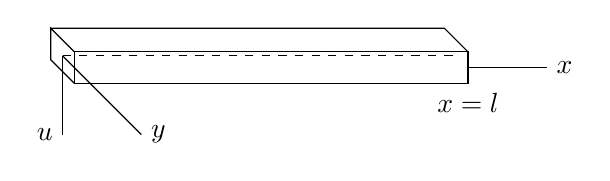
\begin{tikzpicture}[x={(1cm,0)},y={(0.5cm,-0.5cm)},z={(0,1cm)}]
\pgfmathsetmacro{\ax}{5}
\pgfmathsetmacro{\by}{0.6}
\pgfmathsetmacro{\cz}{0.4}
%
\draw(0,0,0)--++(0,0,\cz);
\draw(0,0,0)--++(0,-\by,0)--++(0,0,\cz)--++(0,\by);
\draw(0,0,0)--++(\ax,0,0)--++(0,0,\cz)coordinate(kR)--++(-\ax,0,0);
\draw(kR)--++(0,-\by,0)--++(-\ax,0,0);
%
\draw(\ax,0,1/2*\cz)--++(1,0,0)node[right]{$x$};
\draw(0,-\by/2,\cz/2)--++(0,2,0)node[right]{$y$};
\draw(0,-\by/2,\cz/2)--++(0,0,-1)node[left]{$u$};
\draw[dashed](0,-\by/2,\cz/2)--++(\ax,0,0);
\draw(\ax,0,0)node[below]{$x=l$};
\end{tikzpicture}
\caption*{(الف) شہتیر کی ساخت}
\end{subfigure}
%
\begin{subfigure}{1\textwidth}
\centering
\begin{tikzpicture}
\draw(0,0) to [out=-10,in=-170] (5,0)--++(0,0.4) to [out=-170,in=-10] (0,0.4)--(0,0);
\draw[dashed](0,0.2)node[solid,ocirc]{}--++(5,0);
\draw(5,0.2)--++(1,0)node[right]{$x$};
\draw(0,0)--++(0.3,-0.3)--++(-0.6,0)coordinate(kkL)--++(0.3,0.3);
\draw(5,0)--++(0.3,-0.3)coordinate(kR)--++(-0.6,0)coordinate(kL)--++(0.3,0.3);
\draw(kL)++(2pt,-2pt) node[ocirc]{};
\draw(kR)++(-2pt,-2pt) node[ocirc]{};
\draw[fill=gray!50!white](kkL)--++(-0.25,0)--++(0,-0.2)--++(1.1,0)--++(0,0.2)--++(-1.1,0);
\draw[fill=gray!50!white](kL)++(0,-4pt)--++(-0.25,0)--++(0,-0.2)--++(1.1,0)--++(0,0.2)--++(-1.1,0);
\draw[-latex](0,-0.6)--++(0,-0.75)node[left]{$u$};
\draw(5,-0.6)node[below]{$x=l$};
\end{tikzpicture}
\caption*{(ب) شہتیر کے سر آزاد پڑے ہیں}
\end{subfigure}
%
\begin{subfigure}{1\textwidth}
\centering
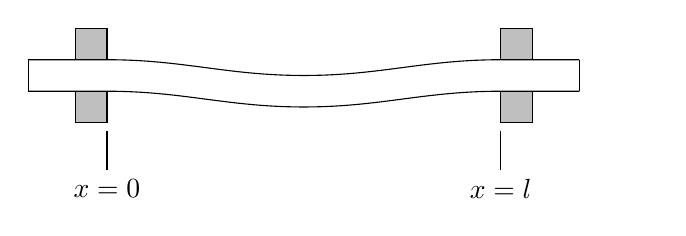
\begin{tikzpicture}
\draw(0,0)--++(1,0) to [out=0,in=180] ++(2.5,-0.2) to [out=0,in=180]++(2.5,0.2) --++(1,0);
\draw(0,0.4)--++(1,0) to [out=0,in=180] ++(2.5,-0.2) to [out=0,in=180]++(2.5,0.2) --++(1,0);
\draw(0,0)--++(0,0.4);
\draw(7,0)--++(0,0.4);
%
\draw[fill=gray!50!white](1,0)--++(0,-0.4)--++(-0.4,0)--++(0,0.4)--++(0.4,0);
\draw[fill=gray!50!white](1,0.4+0.4)--++(0,-0.4)--++(-0.4,0)--++(0,0.4)--++(0.4,0);
%
\draw[fill=gray!50!white](6.4,0)--++(0,-0.4)--++(-0.4,0)--++(0,0.4)--++(0.4,0);
\draw[fill=gray!50!white](6.4,0.4+0.4)--++(0,-0.4)--++(-0.4,0)--++(0,0.4)--++(0.4,0);
%
\draw(1,-0.5)--++(0,-0.5) node[below]{$x=0$};
\draw(6,-0.5)--++(0,-0.5)node[below]{$x=l$};
\path(7,0)--++(1,0);
\end{tikzpicture}
\caption*{(پ) شہتیر کے سر جکڑے ہیں}
\end{subfigure}
\caption{شہتیر کی لرزش}
\label{شکل_جزوی_شہتیر}
\end{figure}
\انتہا{سوال}
%=========================
\ابتدا{سوال}\شناخت{سوال_جزوی_شہتیر_ب}\quad
ابتدائی رفتار صفر لیتے ہوئے  مساوات \حوالہ{مساوات_جزوی_شہتیر_الف} کے وہ حل \عددی{u_n=F_n(x)G_n(t)} دریافت کریں جو درج ذیل ابتدائی شرائط کو مطمئن کرتے ہوں (شکل \حوالہ{شکل_جزوی_شہتیر}-ب)۔
\begin{align*}
u(0,t)&=0,\quad u(l,t)=0 \quad \text{\RL{شہتیر کے دونوں سر دیوار پر آزاد رکھے گئے ہیں}}\\
u_{xx}(0,t)&=0,\quad u_{xx}(l,t)=0\quad \text{\RL{یوں سروں پر صفر معیار اثر لہٰذا صفر گولائی ہو گی}}
\end{align*} 
جواب:\quad
\begin{align*}
F_n=\sin \frac{n\pi x}{l}, \quad G_n=a_n\cos \frac{cn^2\pi^2 t}{l^2}
\end{align*}
\انتہا{سوال}
%===========================
\ابتدا{سوال}\شناخت{سوال_جزوی_شہتیر_پ}\quad
مساوات \حوالہ{مساوات_جزوی_شہتیر_الف} کا وہ حل جو سوال \حوالہ{سوال_جزوی_شہتیر_ب} کے شرائط کے ساتھ ساتھ ابتدائی انحراف \عددی{u(x,0)=f(x)=x(l-x)} کو مطمئن کرتا ہو حاصل کریں۔
\انتہا{سوال}
%==========================
\ابتدا{سوال}\شناخت{سوال_جزوی_شہتیر_ت}\quad
شہتیر کے دونوں سروں سے جکڑنے سے کیا ابتدائی شرائط پیدا ہوں گے (شکل \حوالہ{شکل_جزوی_شہتیر}-پ)؟\\
جواب:\quad
$u(0,t)=0,\quad u(l,0)=0,\quad u_x(0,t)=0,\quad u_x(l,t)=0$
\انتہا{سوال}
%===========================
\ابتدا{سوال}\شناخت{سوال_جزوی_شہتیر_ٹ}\quad
تصدیق کریں کہ سوال \حوالہ{سوال_جزوی_شہتیر_الف} میں حاصل \عددی{F(x)} سوال \حوالہ{سوال_جزوی_شہتیر_ت} میں دی گئی شرائط کو اس صورت مطمئن کرتا ہے جب \عددی{\beta l} درج ذیل مساوات کے جذر ہوں۔
\begin{align}\label{مساوات_جزوی_شہتیر_ب}
\cosh \beta l\cos \beta l=1
\end{align}
مساوات \حوالہ{مساوات_جزوی_شہتیر_ب} کے چند حل کا تخمینہ لگائیں ۔
\انتہا{سوال}
%===========================

\حصہ{یک بعدی بہاو حرارت}
